\documentclass[11pt,a4paper]{article}

% ─── Geometry ───────────────────────────────────────────────────────
\usepackage[top=25mm,bottom=25mm,left=25mm,right=25mm]{geometry}

% ─── Encoding & fonts ──────────────────────────────────────────────
\usepackage[utf8]{inputenc}
\usepackage[T1]{fontenc}
\usepackage{lmodern}
\usepackage{microtype}

% ─── Colour (Rusty Givens palette) ────────────────────────────────
\usepackage{xcolor}
\definecolor{rgblue}{HTML}{003B5C}
\definecolor{rgorange}{HTML}{E67E22}
\definecolor{rggraphite}{HTML}{2C3E50}
\definecolor{rgsilver}{HTML}{ECF0F1}
\definecolor{rgtext}{HTML}{1a2b38}

% ─── Maths ─────────────────────────────────────────────────────────
\usepackage{amsmath,amssymb,bm}

% ─── Tables ────────────────────────────────────────────────────────
\usepackage{booktabs}
\usepackage{tabularx}
\usepackage{longtable}
\usepackage{multirow}
\usepackage{array}

% ─── Graphics ──────────────────────────────────────────────────────
\usepackage{graphicx}
\graphicspath{{figures/}}

% ─── TikZ for diagrams ────────────────────────────────────────────
\usepackage{tikz}
\usetikzlibrary{arrows.meta,positioning,shapes.geometric,fit,calc,backgrounds}

% ─── Code listings ─────────────────────────────────────────────────
\usepackage{listings}
\lstset{
  basicstyle=\ttfamily\small,
  keywordstyle=\color{rgblue}\bfseries,
  commentstyle=\color{rggraphite}\itshape,
  stringstyle=\color{rgorange},
  breaklines=true,
  frame=single,
  rulecolor=\color{rgsilver},
  backgroundcolor=\color{rgsilver!30},
  numbers=left,
  numberstyle=\tiny\color{rggraphite},
}
\lstdefinelanguage{json}{
  morestring=[b]",
  literate=
   *{:}{{{\color{rggraphite}:}}}{1}
    {,}{{{\color{rggraphite},}}}{1}
    {\{}{{{\color{rgblue}\{}}}{1}
    {\}}{{{\color{rgblue}\}}}}{1}
    {[}{{{\color{rgblue}[}}}{1}
    {]}{{{\color{rgblue}]}}}{1}
}

% ─── Hyperlinks ────────────────────────────────────────────────────
\usepackage[hidelinks,colorlinks=true,linkcolor=rgblue,citecolor=rgblue,urlcolor=rgorange]{hyperref}

% ─── Section styling ──────────────────────────────────────────────
\usepackage{titlesec}
\titleformat{\section}{\Large\bfseries\color{rgblue}}{\thesection}{1em}{}
\titleformat{\subsection}{\large\bfseries\color{rggraphite}}{\thesubsection}{1em}{}
\titleformat{\subsubsection}{\normalsize\bfseries\color{rggraphite}}{\thesubsubsection}{1em}{}

% ─── Header / Footer ──────────────────────────────────────────────
\usepackage{fancyhdr}
\pagestyle{fancy}
\fancyhf{}
\renewcommand{\headrulewidth}{0.4pt}
\renewcommand{\footrulewidth}{0.4pt}
\fancyhead[L]{\small\color{rggraphite}Rusty Givens --- Product Description}
\fancyhead[R]{\small\color{rggraphite}\thepage}
\fancyfoot[C]{\small\color{rggraphite}Confidential}

% ─── Enumerations ─────────────────────────────────────────────────
\usepackage{enumitem}
\setlist{nosep,leftmargin=1.5em}

% ─── Bibliography ─────────────────────────────────────────────────
\usepackage[numbers,sort&compress]{natbib}

% ─── Acronyms ─────────────────────────────────────────────────────
\usepackage[acronym,toc,nonumberlist]{glossaries}
\makeglossaries
% Acronym definitions for glossaries package

\newacronym{WLS}{WLS}{Weighted Least Squares}
\newacronym{SE}{SE}{State Estimation}
\newacronym{OA}{OA}{Observability Analysis}
\newacronym{BDD}{BDD}{Bad Data Detection}
\newacronym{KKT}{KKT}{Karush--Kuhn--Tucker}
\newacronym{PMU}{PMU}{Phasor Measurement Unit}
\newacronym{API}{API}{Application Programming Interface}
\newacronym{REST}{REST}{Representational State Transfer}
\newacronym{gRPC}{gRPC}{Google Remote Procedure Call}
\newacronym{GB}{GB}{Great Britain}
\newacronym{EHV}{EHV}{Extra High Voltage}
\newacronym{TSO}{TSO}{Transmission System Operator}
\newacronym{RTU}{RTU}{Remote Terminal Unit}
\newacronym{SCADA}{SCADA}{Supervisory Control and Data Acquisition}
\newacronym{DC}{DC}{Direct Current}
\newacronym{AC}{AC}{Alternating Current}
\newacronym{QR}{QR}{QR Decomposition}
\newacronym{LU}{LU}{LU Decomposition}
\newacronym{LLT}{LLT}{Cholesky Decomposition}
\newacronym{ZI}{ZI}{Zero Injection}
\newacronym{MAE}{MAE}{Mean Absolute Error}
\newacronym{JSON}{JSON}{JavaScript Object Notation}
\newacronym{CSV}{CSV}{Comma-Separated Values}
\newacronym{GNN}{GNN}{Graph Neural Network}
\newacronym{ONNX}{ONNX}{Open Neural Network Exchange}


% ─── Document metadata ────────────────────────────────────────────
\title{%
  \vspace{-1cm}
  {\color{rgorange}\rule{\textwidth}{2pt}}\\[0.4cm]
  {\Huge\bfseries\color{rgblue}Rusty Givens}\\[0.2cm]
  {\Large\color{rggraphite}Product Description}\\[0.1cm]
  {\large\color{rggraphite}Modular Power System State Estimator}\\[0.3cm]
  {\color{rgorange}\rule{\textwidth}{2pt}}
}
\author{}
\date{\today}

% ═══════════════════════════════════════════════════════════════════
\begin{document}
\maketitle
\thispagestyle{empty}

\vspace{1cm}
\begin{center}
\begin{tabular}{ll}
  \toprule
  \textbf{Document type}  & Product Description (Technical) \\
  \textbf{Audience}        & Subject Matter Experts, Domain Architects \\
  \textbf{Edition}         & Pro (includes all Free-edition features) \\
  \textbf{Implementation language} & Rust 1.75+ \\
  \textbf{License (Free)}  & Apache 2.0 \\
  \textbf{License (Pro)}   & Commercial \\
  \textbf{Version}         & 0.1.0 \\
  \bottomrule
\end{tabular}
\end{center}

\clearpage
\tableofcontents
\clearpage


% ═══════════════════════════════════════════════════════════════════
%  PART I — OVERVIEW
% ═══════════════════════════════════════════════════════════════════

\section{Introduction}\label{sec:intro}

Rusty Givens is a modular AC Weighted Least Squares (\gls{WLS}) state
estimator written in Rust.  It addresses the need for transparent,
high-performance, and vendor-independent implementations of the classical
\gls{SE} pipeline as articulated by ENTSO-E~\cite{entsoe2025}:
measurement modelling, observability analysis, state estimation, bad data
detection, and redundancy analysis.

The implementation follows the mathematical framework of Abur and
Exp\'{o}sito~\cite{abur2004} and Monticelli~\cite{monticelli1999}.  The
software is distributed in two editions:

\begin{description}[style=nextline]
  \item[Free Edition (Apache 2.0)]
    SE kernel with six solver formulations, three factorisations,
    six measurement types, measurement metadata and flags, zero-injection
    handling, a substitution value framework with priority resolution,
    voltage averaging, sigma statistics, post-estimation evaluation,
    REST and gRPC APIs, an Angular frontend, and a full Great Britain
    transmission network case study.
  \item[Pro Edition (Commercial)]
    All Free-edition features plus Observability Analysis (numerical
    and topological), Redundancy Analysis (sensitivity-matrix-based
    measurement classification with Good/Bad marks), and Bad Data
    Detection (chi-squared test, residual-based identification, iterative
    elimination, Givens compensation, measurement lifecycle management).
\end{description}

This document describes both editions in the detail required by
power-system subject-matter experts evaluating the mathematical rigour and
feature completeness, and by domain architects evaluating deployment
topology, API contracts, and integration patterns.


% ═══════════════════════════════════════════════════════════════════
%  PART II — ARCHITECTURE (Domain Architect focus)
% ═══════════════════════════════════════════════════════════════════

\section{System Architecture}\label{sec:arch}

\subsection{Design principles}

\begin{enumerate}
  \item \textbf{Library-first.}  All mathematical algorithms live in pure
        Rust library crates with no I/O, no network, and no side effects.
        They can be embedded into any Rust application, including
        Kubernetes operators and serverless functions.
  \item \textbf{Separation of concerns.}  The I/O layer, the HTTP/gRPC
        service, and the frontend are separate compilation units.  A
        change in the API serialisation format does not require recompiling
        the SE kernel.
  \item \textbf{Conditional compilation.}  Pro crates are optional
        dependencies gated behind a Cargo feature flag
        (\texttt{--features pro}).  The estimate service compiles and
        functions without them.
  \item \textbf{Zero-copy shared state.}  The service holds a single
        \texttt{Arc<AppState>} that is shared across all request handlers.
        Mutable state (last result, BDD state, substitution set) is
        protected by \texttt{tokio::sync::Mutex}.
  \item \textbf{Dual API.}  Every computational capability is exposed via
        both a JSON/REST interface (for browser clients and scripting)
        and a Protobuf/gRPC interface (for inter-service communication and
        high-throughput pipelines).
\end{enumerate}

\subsection{Workspace layout}

The Cargo workspace (resolver v2) contains the following members:

\begin{center}
\small
\begin{tabular}{lllp{48mm}}
  \toprule
  \textbf{Component} & \textbf{Path} & \textbf{Edition} & \textbf{Role} \\
  \midrule
  SE kernel          & \texttt{crates/rusty-givens-core} & Free
    & Pure math library: network model, AC model, measurement model,
      Jacobian, six solver formulations, post-estimation, ZI, substitution \\
  JSON I/O           & \texttt{crates/rusty-givens-io}   & Free
    & Deserialise JSON case files into core types \\
  Case-study runner  & \texttt{crates/gb-case-study}     & Free
    & CLI binary for batch comparison of formulations \\
  Observability      & \texttt{crates/pro/rusty-givens-obs} & Pro
    & Numerical and topological observability analysis \\
  Redundancy         & \texttt{crates/pro/rusty-givens-red} & Pro
    & Sensitivity-based redundancy classification \\
  Bad Data Detection & \texttt{crates/pro/rusty-givens-bdd} & Pro
    & Chi-squared, residual tests, iterative elimination, lifecycle \\
  Estimate service   & \texttt{services/estimate-service} & Free+Pro
    & Async REST+gRPC service (axum + tonic) \\
  Angular frontend   & \texttt{frontend/}                 & Free
    & Single-page application (Angular 17+) \\
  Protobuf defs      & \texttt{proto/}                    & Free+Pro
    & Interface contract shared between service and clients \\
  \bottomrule
\end{tabular}
\end{center}

\subsection{Dependency graph}

\begin{center}
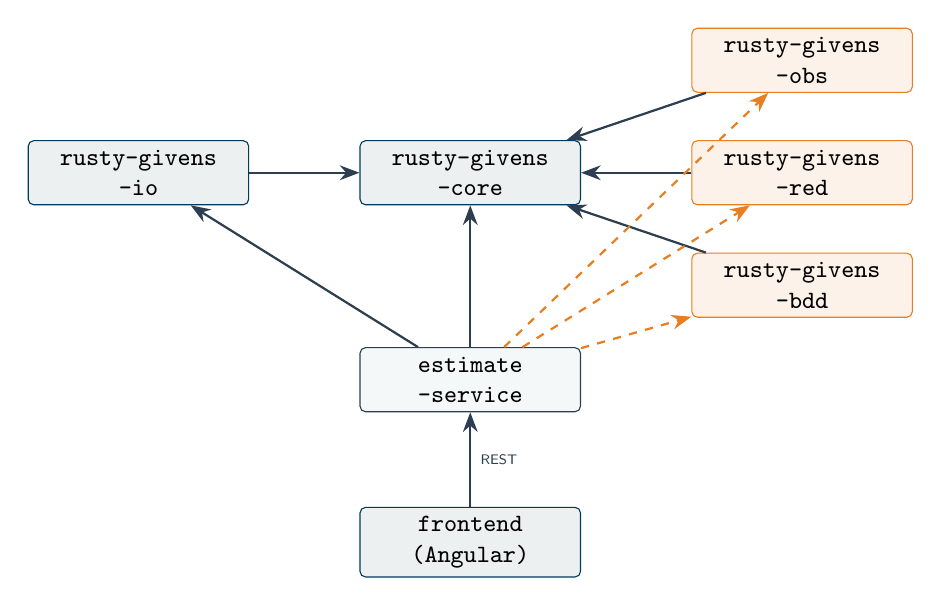
\begin{tikzpicture}[
  crate/.style={draw=rgblue, fill=rgsilver, rounded corners=2pt,
                minimum height=8mm, minimum width=28mm, align=center,
                font=\small\ttfamily},
  procrate/.style={crate, draw=rgorange, fill=rgorange!10},
  svc/.style={draw=rggraphite, fill=rgsilver!50, rounded corners=2pt,
              minimum height=8mm, minimum width=28mm, align=center,
              font=\small\ttfamily},
  arr/.style={-{Stealth[length=2.5mm]}, thick, color=rggraphite},
  node distance=6mm and 14mm
]
  \node[crate] (core) {rusty-givens\\-core};
  \node[crate, left=of core] (io) {rusty-givens\\-io};
  \node[procrate, above right=6mm and 14mm of core] (obs) {rusty-givens\\-obs};
  \node[procrate, right=of core] (red) {rusty-givens\\-red};
  \node[procrate, below right=6mm and 14mm of core] (bdd) {rusty-givens\\-bdd};
  \node[svc, below=18mm of core] (svc) {estimate\\-service};
  \node[crate, below=12mm of svc] (fe) {frontend\\(Angular)};

  \draw[arr] (io) -- (core);
  \draw[arr] (obs) -- (core);
  \draw[arr] (red) -- (core);
  \draw[arr] (bdd) -- (core);
  \draw[arr] (svc) -- (core);
  \draw[arr] (svc) -- (io);
  \draw[arr, dashed, color=rgorange] (svc) -- (obs);
  \draw[arr, dashed, color=rgorange] (svc) -- (red);
  \draw[arr, dashed, color=rgorange] (svc) -- (bdd);
  \draw[arr] (fe) -- node[right,font=\tiny\sffamily]{REST} (svc);
\end{tikzpicture}
\end{center}

\noindent
Dashed orange arrows indicate optional (Pro) dependencies.

\subsection{Third-party dependencies}

\begin{center}
\small
\begin{tabular}{lll}
  \toprule
  \textbf{Crate} & \textbf{Version} & \textbf{Purpose} \\
  \midrule
  \texttt{faer}        & latest & Dense and sparse linear algebra
    (Cholesky, LU, column-pivoted QR) \\
  \texttt{sprs}        & latest & Sparse matrix construction (CSC/CSR)
    and arithmetic \\
  \texttt{num-complex}  & latest & Complex arithmetic for
    $Y_\text{bus}$ assembly \\
  \texttt{axum}        & 0.8    & Async HTTP framework (REST API) \\
  \texttt{tokio}       & 1      & Async runtime (multi-threaded, full
    feature set) \\
  \texttt{tower-http}  & 0.6    & CORS middleware \\
  \texttt{tonic}       & 0.12   & gRPC server \\
  \texttt{prost}       & 0.13   & Protobuf code generation \\
  \texttt{serde / serde\_json} & 1.0 & JSON serialisation \\
  \texttt{statrs}      & latest & Statistical distributions
    (chi-squared CDF, Pro) \\
  \texttt{env\_logger / log} & latest & Structured logging \\
  \bottomrule
\end{tabular}
\end{center}

\subsection{Processing pipeline}\label{sec:pipeline}

\begin{center}
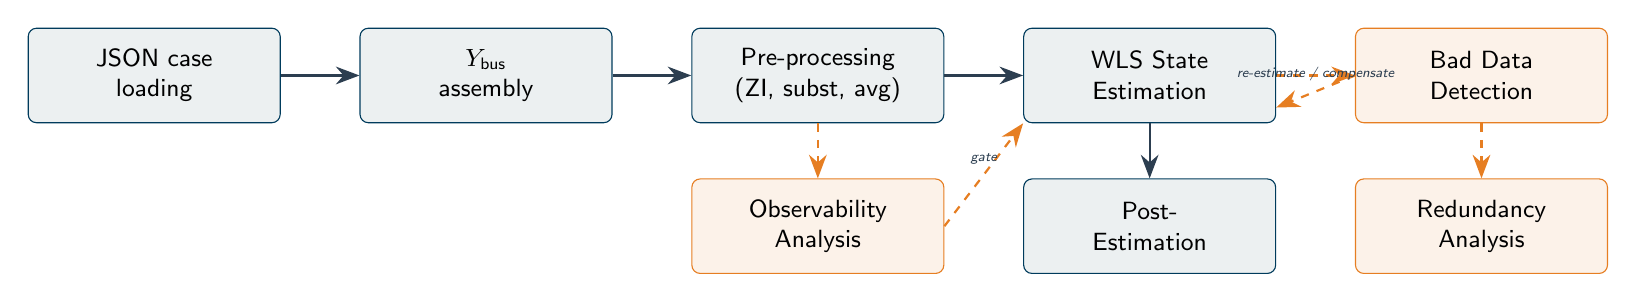
\begin{tikzpicture}[
  block/.style={draw=rgblue, fill=rgsilver, rounded corners=3pt,
                minimum height=12mm, minimum width=32mm, align=center,
                font=\small\sffamily},
  problock/.style={block, draw=rgorange, fill=rgorange!10},
  arr/.style={-{Stealth[length=3mm]}, thick, color=rggraphite},
  darr/.style={-{Stealth[length=3mm]}, thick, dashed, color=rgorange},
  note/.style={font=\tiny\sffamily\itshape, color=rggraphite},
  node distance=7mm and 10mm
]
  \node[block] (load) {JSON case\\loading};
  \node[block, right=of load] (model) {$Y_\text{bus}$\\assembly};
  \node[block, right=of model] (preproc) {Pre-processing\\(ZI, subst, avg)};
  \node[problock, below=of preproc] (oa) {Observability\\Analysis};
  \node[block, right=of preproc] (se) {WLS State\\Estimation};
  \node[block, below=of se] (post) {Post-\\Estimation};
  \node[problock, right=of se] (bdd) {Bad Data\\Detection};
  \node[problock, below=of bdd] (red) {Redundancy\\Analysis};

  \draw[arr] (load) -- (model);
  \draw[arr] (model) -- (preproc);
  \draw[arr] (preproc) -- (se);
  \draw[darr] (preproc) -- (oa);
  \draw[darr] (oa.east) -- node[above,note]{gate} (se.south west);
  \draw[arr] (se) -- (post);
  \draw[darr] (se) -- (bdd);
  \draw[darr] (bdd) -- (red);
  \draw[darr] (bdd.west) -- node[above,note]{re-estimate / compensate}
    ([yshift=2mm]se.south east);
\end{tikzpicture}
\end{center}

\noindent
Orange blocks are Pro-only.  Within the pre-processing stage, the following
steps execute in order: (1)~substitution sigma adjustment, (2)~voltage
averaging, (3)~zero-injection virtual measurement injection.  The pipeline
can be executed end-to-end via a single API call or invoked step by step
through individual endpoints.


\subsection{Concurrency model}

The estimate service runs on the Tokio multi-threaded async runtime.  Each
inbound HTTP or gRPC request spawns a task on the Tokio thread pool.  The
SE solver itself is CPU-bound and executed synchronously within the task;
\texttt{spawn\_blocking} is not currently used because typical SE wall-clock
time ($<100$\,ms for the GB network) is below the threshold where yielding
to the executor would provide measurable benefit.

Shared mutable state is held in \texttt{Arc<AppState>} with individual
\texttt{Mutex} guards per field:

\begin{center}
\small
\begin{tabular}{lp{65mm}}
  \toprule
  \textbf{Field} & \textbf{Description} \\
  \midrule
  \texttt{last\_result}             & Last \texttt{SeResultPayload} (JSON-ready) \\
  \texttt{last\_se\_result}         & Last \texttt{EstimationResult} (typed, for BDD input) \\
  \texttt{substitution\_set}        & Uploaded substitution values \\
  \texttt{bdd\_state}               & Lifecycle counters, bad data / historical sets (Pro) \\
  \texttt{last\_bdd\_artifacts}     & Solver artifacts from last BDD re-estimation (Pro) \\
  \texttt{last\_bdd\_measurements}  & Measurement set after BDD eliminations (Pro) \\
  \bottomrule
\end{tabular}
\end{center}

\noindent
Immutable data (network topology, AC model, base measurements, true state,
bus metadata) is shared without a lock.

\subsection{Build system and feature gating}

The workspace uses Cargo with resolver v2.  The estimate service declares
the Pro crates as optional dependencies:

\begin{lstlisting}[language={}]
[features]
default = []
pro = [
  "dep:rusty-givens-bdd",
  "dep:rusty-givens-obs",
  "dep:rusty-givens-red",
]
\end{lstlisting}

Building the Free edition requires only \texttt{cargo build --release}.
Building the Pro edition requires \texttt{cargo build --release --features pro}.
Code that references Pro types is guarded by \texttt{\#[cfg(feature = "pro")]}.

\subsection{Containerisation and deployment}\label{sec:deploy}

No Dockerfile is shipped in the current release.  The recommended
container strategy is:

\begin{enumerate}
  \item \textbf{Multi-stage build.}  Stage~1: \texttt{rust:1.75-bookworm}
        compiles the release binary.  Stage~2: \texttt{debian:bookworm-slim}
        copies the binary and the case file.
  \item \textbf{Ports.}  REST on \texttt{3001/tcp}, gRPC on
        \texttt{50051/tcp}.
  \item \textbf{Health check.}  \texttt{GET /api/network} returns
        \texttt{200~OK} with the topology; suitable as a liveness and
        readiness probe.
  \item \textbf{Configuration.}  Case file path via environment variable
        or volume mount.  All SE parameters are per-request; no server-side
        configuration file is required.
  \item \textbf{Frontend.}  The Angular application is a static build
        (\texttt{ng build --configuration production}) served by any
        HTTP server (nginx, Caddy).  A dev-mode proxy routes
        \texttt{/api/*} to \texttt{http://localhost:3001}.
  \item \textbf{Horizontal scaling.}  The service is stateless per network;
        each instance loads its own case file.  Instances can be
        load-balanced behind a reverse proxy.  BDD lifecycle state is
        instance-local; for multi-instance deployments, an external state
        store (Redis, PostgreSQL) would be required.
\end{enumerate}

\begin{center}
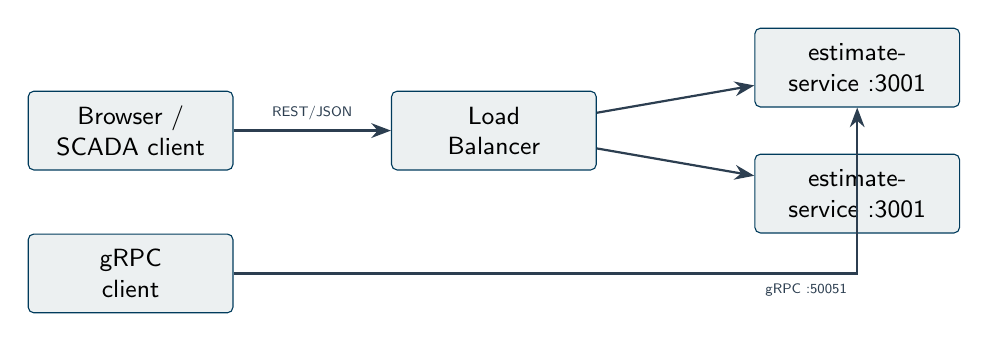
\begin{tikzpicture}[
  box/.style={draw=rgblue, fill=rgsilver, rounded corners=2pt,
              minimum height=10mm, minimum width=26mm, align=center,
              font=\small\sffamily},
  arr/.style={-{Stealth[length=2.5mm]}, thick, color=rggraphite},
  node distance=8mm and 10mm
]
  \node[box] (client) {Browser /\\SCADA client};
  \node[box, right=20mm of client] (lb) {Load\\Balancer};
  \node[box, right=20mm of lb, yshift=8mm] (svc1) {estimate-\\service :3001};
  \node[box, right=20mm of lb, yshift=-8mm] (svc2) {estimate-\\service :3001};
  \node[box, below=of client] (grpc) {gRPC\\client};

  \draw[arr] (client) -- node[above,font=\tiny\sffamily]{REST/JSON} (lb);
  \draw[arr] (lb) -- (svc1);
  \draw[arr] (lb) -- (svc2);
  \draw[arr] (grpc) -| node[below left,font=\tiny\sffamily]{gRPC :50051} (svc1);
\end{tikzpicture}
\end{center}

\subsection{Startup sequence}

\begin{enumerate}
  \item Initialise \texttt{env\_logger}.
  \item Load the JSON case file via \texttt{rusty\_givens\_io::load\_case}.
  \item Build the AC model ($Y_\text{bus}$, $G_\text{bus}$, $B_\text{bus}$,
        per-branch parameters).
  \item Construct \texttt{AppState} (immutable topology + Mutex-wrapped
        mutable fields).
  \item Wrap in \texttt{Arc} and attach to both routers.
  \item Spawn REST server on \texttt{0.0.0.0:3001} (axum) and gRPC server
        on \texttt{0.0.0.0:50051} (tonic) concurrently via
        \texttt{tokio::select!}.
\end{enumerate}


% ═══════════════════════════════════════════════════════════════════
%  PART III — NETWORK MODEL (SE Expert focus)
% ═══════════════════════════════════════════════════════════════════

\section{Network Model}\label{sec:network}

\subsection{Bus representation}

Each bus is characterised by the following attributes, stored in the
\texttt{Bus} struct:

\begin{center}
\small
\begin{tabular}{llll}
  \toprule
  \textbf{Field} & \textbf{Rust type} & \textbf{Unit} & \textbf{Description} \\
  \midrule
  \texttt{label}             & \texttt{usize} & --- & Unique identifier \\
  \texttt{bus\_type}          & \texttt{BusType} & --- &
    \texttt{PQ} (1), \texttt{PV} (2), \texttt{Slack} (3) \\
  \texttt{active\_demand}     & \texttt{f64}   & p.u. & Scheduled $P_\text{load}$ \\
  \texttt{reactive\_demand}   & \texttt{f64}   & p.u. & Scheduled $Q_\text{load}$ \\
  \texttt{shunt\_conductance} & \texttt{f64}   & p.u. & $G_\text{sh}$ \\
  \texttt{shunt\_susceptance} & \texttt{f64}   & p.u. & $B_\text{sh}$ \\
  \texttt{voltage\_magnitude} & \texttt{f64}   & p.u. & Initial guess $V^{(0)}$ \\
  \texttt{voltage\_angle}     & \texttt{f64}   & rad  & Initial guess $\theta^{(0)}$ \\
  \bottomrule
\end{tabular}
\end{center}

\noindent
Bus metadata (nominal voltage $V_n$ in kV, geographic coordinates
\texttt{geo\_x}, \texttt{geo\_y}) is stored separately in
\texttt{BusMetadata} and used for per-voltage-level reporting and
frontend visualisation.

\subsection{Branch $\pi$-model}\label{sec:pi}

Each branch is represented by the standard $\pi$-equivalent circuit with
tap and phase shifter:

\begin{center}
\small
\begin{tabular}{llll}
  \toprule
  \textbf{Field} & \textbf{Rust type} & \textbf{Unit} & \textbf{Description} \\
  \midrule
  \texttt{label}        & \texttt{usize} & --- & Unique identifier \\
  \texttt{from / to}    & \texttt{usize} & --- & Terminal bus indices \\
  \texttt{resistance}   & \texttt{f64}   & p.u. & Series resistance $R$ \\
  \texttt{reactance}    & \texttt{f64}   & p.u. & Series reactance $X$ \\
  \texttt{susceptance}  & \texttt{f64}   & p.u. & Total charging $B_c$ \\
  \texttt{conductance}  & \texttt{f64}   & p.u. & Shunt conductance $G_c$ \\
  \texttt{tap\_ratio}   & \texttt{f64}   & --- & Off-nominal tap $\tau$ \\
  \texttt{shift\_angle} & \texttt{f64}   & rad  & Phase shift $\varphi$ \\
  \texttt{status}       & \texttt{bool}  & --- & In service / out of service \\
  \bottomrule
\end{tabular}
\end{center}

\noindent
The $2\times2$ branch admittance matrix for branch $(i,j)$ is:

\begin{equation}\label{eq:ybranch}
  \mathbf{Y}_\text{branch} =
  \begin{bmatrix}
    \dfrac{y_s + y_c}{\tau^2}
    & -\dfrac{y_s}{\tau\,e^{-j\varphi}} \\[6pt]
    -\dfrac{y_s}{\tau\,e^{j\varphi}}
    & y_s + y_c
  \end{bmatrix}
\end{equation}

\noindent
where the series admittance is $y_s = g + jb = 1/(R + jX)$ and the shunt
admittance is $y_c = G_c/2 + jB_c/2$.

\subsection{Bus admittance matrix $Y_\text{bus}$}\label{sec:ybus}

The $n \times n$ bus admittance matrix is assembled from branch
contributions and bus shunt elements.  For each in-service branch
$(i,j)$, define the complex tap factor
$\alpha = (\cos\varphi - j\sin\varphi)/\tau$.  Then:

\begin{align}
  Y_{ii}  &\mathrel{+}= \frac{y_s + y_c}{\tau^2}
  &\quad& Y_{jj} \mathrel{+}= y_s + y_c \notag \\
  Y_{ij}  &\mathrel{+}= -\bar{\alpha}\,y_s
  &\quad& Y_{ji} \mathrel{+}= -\alpha\,y_s
\end{align}

\noindent
Bus shunt contributions add $G_\text{sh} + jB_\text{sh}$ to the
diagonal.  The real and imaginary parts are extracted as:

\begin{equation}
  G_\text{bus} = \operatorname{Re}(Y_\text{bus}), \qquad
  B_\text{bus} = \operatorname{Im}(Y_\text{bus})
\end{equation}

\noindent
All three matrices are stored in compressed sparse column (CSC) format
via \texttt{sprs}.  The AC model also pre-computes per-branch parameters
$(g, b, g_s, b_s, \tau, \varphi)$ for use in the Jacobian evaluator.

\subsection{Per-branch derived parameters}\label{sec:branchparams}

For each branch, the following derived quantities are used in branch flow
and current magnitude computations:

\begin{align}
  g_s &= G_c / 2 & b_s &= B_c / 2 \notag \\
  A_\text{from} &= \frac{(g+g_s)^2 + (b+b_s)^2}{\tau^4}
  & B_\text{from} &= \frac{g^2 + b^2}{\tau^2} \notag \\
  C_\text{from} &= \frac{g(g+g_s) + b(b+b_s)}{\tau^3}
  & D_\text{from} &= \frac{g\,b_s - b\,g_s}{\tau^3}
\end{align}

\noindent
Symmetric expressions hold for the ``to'' end with the appropriate powers
of $\tau$.


% ═══════════════════════════════════════════════════════════════════
%  PART IV — MEASUREMENT MODELLING
% ═══════════════════════════════════════════════════════════════════

\section{Measurement Modelling}\label{sec:meas}

\subsection{State vector convention}

The state vector has dimension $n_s = 2n - 1$ (the slack bus angle is
fixed at its initial value):
\begin{equation}
  \mathbf{x} = [\theta_1, \ldots, \theta_n, V_1, \ldots, V_n]^T
\end{equation}
Column indices $0, \ldots, n{-}1$ correspond to angles; indices $n, \ldots,
2n{-}1$ correspond to voltage magnitudes.  The Jacobian column for the
slack bus angle is zeroed.

\subsection{Supported measurement types and functions}

\subsubsection{Voltmeter (bus voltage magnitude)}

\begin{equation}
  h_V(i) = V_i, \qquad
  \frac{\partial h}{\partial V_i} = 1
\end{equation}

\subsubsection{Wattmeter --- bus injection}

\begin{equation}
  h_{P_i}(\mathbf{x}) = V_i \sum_{j=1}^{n}
    \bigl(G_{ij}\cos\theta_{ij} + B_{ij}\sin\theta_{ij}\bigr)\,V_j
\end{equation}

Jacobian entries for $j \neq i$:
\begin{align}
  \frac{\partial h_{P_i}}{\partial \theta_i} &=
    V_i \sum_{j} (-G_{ij}\sin\theta_{ij} + B_{ij}\cos\theta_{ij})\,V_j
    - B_{ii}\,V_i^2 \\
  \frac{\partial h_{P_i}}{\partial \theta_j} &=
    (G_{ij}\sin\theta_{ij} - B_{ij}\cos\theta_{ij})\,V_i\,V_j \\
  \frac{\partial h_{P_i}}{\partial V_i} &=
    \sum_{j} (G_{ij}\cos\theta_{ij} + B_{ij}\sin\theta_{ij})\,V_j
    + G_{ii}\,V_i \\
  \frac{\partial h_{P_i}}{\partial V_j} &=
    (G_{ij}\cos\theta_{ij} + B_{ij}\sin\theta_{ij})\,V_i
\end{align}

\subsubsection{Wattmeter --- branch flow (from terminal)}

Let $\theta_{tp} = \theta_i - \theta_j - \varphi$ and use the parameters
from Section~\ref{sec:branchparams}:

\begin{equation}
  h_{P_{ij}}^\text{from} =
    \frac{g + g_s}{\tau^2}\,V_i^2
    - \frac{1}{\tau}(g\cos\theta_{tp} + b\sin\theta_{tp})\,V_i\,V_j
\end{equation}

\begin{align}
  \frac{\partial h}{\partial \theta_i} &=
    \tfrac{1}{\tau}(g\sin\theta_{tp} - b\cos\theta_{tp})\,V_i\,V_j
  &\quad \frac{\partial h}{\partial \theta_j} &= -\frac{\partial h}{\partial \theta_i}
  \\
  \frac{\partial h}{\partial V_i} &=
    \tfrac{2(g+g_s)}{\tau^2}\,V_i - \tfrac{1}{\tau}(g\cos\theta_{tp} +
    b\sin\theta_{tp})\,V_j
  &\quad \frac{\partial h}{\partial V_j} &=
    -\tfrac{1}{\tau}(g\cos\theta_{tp} + b\sin\theta_{tp})\,V_i
\end{align}

\noindent
The ``to'' terminal expression swaps the role of $V_i$ and $V_j$ and
adjusts the sign of the $\sin\theta_{tp}$ term.

\subsubsection{Varmeter --- bus injection}

\begin{equation}
  h_{Q_i}(\mathbf{x}) = V_i \sum_{j=1}^{n}
    \bigl(G_{ij}\sin\theta_{ij} - B_{ij}\cos\theta_{ij}\bigr)\,V_j
\end{equation}

Jacobian entries:
\begin{align}
  \frac{\partial h_{Q_i}}{\partial \theta_i} &=
    V_i \sum_{j} (G_{ij}\cos\theta_{ij} + B_{ij}\sin\theta_{ij})\,V_j
    - G_{ii}\,V_i^2 \\
  \frac{\partial h_{Q_i}}{\partial \theta_j} &=
    -(G_{ij}\cos\theta_{ij} + B_{ij}\sin\theta_{ij})\,V_i\,V_j \\
  \frac{\partial h_{Q_i}}{\partial V_i} &=
    \sum_{j} (G_{ij}\sin\theta_{ij} - B_{ij}\cos\theta_{ij})\,V_j
    - B_{ii}\,V_i \\
  \frac{\partial h_{Q_i}}{\partial V_j} &=
    (G_{ij}\sin\theta_{ij} - B_{ij}\cos\theta_{ij})\,V_i
\end{align}

\subsubsection{Varmeter --- branch flow (from terminal)}

\begin{equation}
  h_{Q_{ij}}^\text{from} =
    -\frac{b + b_s}{\tau^2}\,V_i^2
    - \frac{1}{\tau}(g\sin\theta_{tp} - b\cos\theta_{tp})\,V_i\,V_j
\end{equation}

Jacobian entries follow the same structure as the wattmeter branch flow
with the appropriate substitution of $g$ and $b$ coefficients.

\subsubsection{Ammeter (branch current magnitude)}

Using the branch current magnitude squared:

\begin{equation}
  |I_{ij}|^2 = A\,V_i^2 + B\,V_j^2
    - 2\bigl[C\cos(\theta_{ij}{-}\varphi) \mp D\sin(\theta_{ij}{-}\varphi)\bigr]
    V_i\,V_j
\end{equation}

\noindent
where $A$, $B$, $C$, $D$ are the per-branch derived parameters and the
sign convention depends on the terminal (from/to).  The measurement
function is $h = \sqrt{|I_{ij}|^2}$ by default, or $h = |I_{ij}|^2$ in
squared mode.  In the non-squared case, the Jacobian is divided by
$2\,|I_{ij}|$.

\subsubsection{PMU --- bus (polar coordinates)}

\begin{align}
  h_V &= V_i, &\quad \frac{\partial h_V}{\partial V_i} &= 1 \\
  h_\theta &= \theta_i, &\quad \frac{\partial h_\theta}{\partial \theta_i} &= 1
\end{align}

\subsubsection{PMU --- bus (rectangular coordinates)}

\begin{align}
  h_\text{Re} &= V_i\cos\theta_i
  & h_\text{Im} &= V_i\sin\theta_i \\
  \frac{\partial h_\text{Re}}{\partial \theta_i} &= -V_i\sin\theta_i
  & \frac{\partial h_\text{Re}}{\partial V_i} &= \cos\theta_i \\
  \frac{\partial h_\text{Im}}{\partial \theta_i} &= V_i\cos\theta_i
  & \frac{\partial h_\text{Im}}{\partial V_i} &= \sin\theta_i
\end{align}

\noindent
Variance propagation for rectangular coordinates:
\begin{align}
  \sigma_\text{Re}^2 &= \sigma_V^2\cos^2\theta + \sigma_\theta^2(z_V\sin\theta)^2 \\
  \sigma_\text{Im}^2 &= \sigma_V^2\sin^2\theta + \sigma_\theta^2(z_V\cos\theta)^2
\end{align}

\noindent
Optional $2\times2$ correlated covariance blocks are supported for PMU
measurements where magnitude and angle errors are correlated.

\subsubsection{PMU --- branch (current phasor)}

For a branch PMU, both current magnitude and current angle $\psi$ are
measured.  The magnitude uses the ammeter measurement function.  The
current angle is computed as:
\begin{equation}
  \psi = \operatorname{atan2}(\text{Im}(I_{ij}),\; \text{Re}(I_{ij}))
\end{equation}
The Jacobian of $\psi$ uses the chain rule:
$\partial\psi/\partial x_k = (-\text{Im}/|I|^2)\,\partial\text{Re}/\partial x_k
  + (\text{Re}/|I|^2)\,\partial\text{Im}/\partial x_k$.

\subsubsection{Current angle meter}

Measures $\angle I_{ij}$ at a branch terminal.  The measurement function
is identical to the PMU branch current angle above.

\subsection{Measurement metadata}\label{sec:meta}

Every measurement carries a \texttt{MeasurementMeta} structure with three
fields:

\begin{center}
\small
\begin{tabular}{llp{62mm}}
  \toprule
  \textbf{Field} & \textbf{Type} & \textbf{Values and semantics} \\
  \midrule
  \texttt{timestamp} & \texttt{Option<f64>} &
    UNIX epoch of the measurement acquisition.  Used to determine old
    measurement validity in the substitution framework. \\
  \texttt{flag} & \texttt{MeasurementFlag} &
    \texttt{Valid} --- real-time telemetry, usable;
    \texttt{Blocked} --- excluded by operator;
    \texttt{Invalid} --- failed plausibility;
    \texttt{Substituted} --- replaced by a substitution value;
    \texttt{Calculated} --- derived from other data;
    \texttt{Estimated} --- produced by SE. \\
  \texttt{source} & \texttt{MeasurementSource} &
    \texttt{Realtime} --- SCADA/RTU;
    \texttt{ManualEntry} --- operator;
    \texttt{External} --- forecast, GNN;
    \texttt{SeInternal} --- SE-generated;
    \texttt{ZeroInjection} --- ZI virtual measurement. \\
  \bottomrule
\end{tabular}
\end{center}

\noindent
Metadata is populated from the JSON case file (optional fields with
defaults) and updated during processing (e.g.\ substitution injection sets
\texttt{flag = Substituted} and \texttt{source} to the corresponding
substitution source).

\subsection{Weighting}\label{sec:weight}

Each measurement is weighted by the inverse of its variance:
\begin{equation}
  w_i = \frac{1}{\sigma_i^2}
\end{equation}
The diagonal weight matrix $W = \operatorname{diag}(w_1, \ldots, w_m)$ is
used in all solver formulations.  Off-diagonal entries $W_{ik}$ are
non-zero only for correlated PMU measurements (rectangular mode).

\subsection{Sigma statistics}\label{sec:sigma-stats}

The system computes per-type, per-voltage-level sigma statistics:

\begin{center}
\small
\begin{tabular}{lp{70mm}}
  \toprule
  \textbf{Metric} & \textbf{Description} \\
  \midrule
  $\sigma_\text{min}$ & Minimum $\sigma$ for this measurement type and voltage level \\
  $\sigma_\text{max}$ & Maximum $\sigma$ for this measurement type and voltage level \\
  Count               & Number of measurements in this group \\
  \bottomrule
\end{tabular}
\end{center}

\noindent
Zero-injection virtual measurements (\texttt{source = ZeroInjection}) are
excluded from the statistics.  Results are available globally per type
and broken down per type--voltage-level combination.

\subsection{Voltage averaging}\label{sec:volt-avg}

When multiple voltmeters measure the same bus, a global configuration
switch selects one of two modes:

\begin{description}
  \item[Individual (\texttt{VoltageAveragingMode::Individual})]
    Each voltmeter is retained as a separate measurement equation.
  \item[Weighted average (\texttt{VoltageAveragingMode::WeightedAverage})]
    For each bus with $k > 1$ voltmeters, a single virtual voltmeter
    replaces the originals:
    \begin{equation}
      \bar{V} = \frac{\sum_{i=1}^{k} V_i / \sigma_i^2}
                     {\sum_{i=1}^{k} 1/\sigma_i^2}, \qquad
      \sigma_\text{avg}^2 = \frac{1}{\sum_{i=1}^{k} 1/\sigma_i^2}
    \end{equation}
    This reduces the measurement count and improves numerical conditioning
    when individual voltmeters have significantly different variances.
\end{description}


% ═══════════════════════════════════════════════════════════════════
%  PART V — SUBSTITUTION VALUE FRAMEWORK
% ═══════════════════════════════════════════════════════════════════

\section{Substitution Value Framework}\label{sec:subst}

When buses lack sufficient measurements---either initially or because
measurements are eliminated during bad data treatment---substitution
values provide soft-weighted fallback data to restore observability.

\subsection{Substitution value types}

Three physical quantities can be substituted:

\begin{center}
\begin{tabular}{ll}
  \toprule
  \textbf{Enum variant} & \textbf{Physical quantity} \\
  \midrule
  \texttt{ActivePower}      & Bus injection $P_i$ (p.u.) \\
  \texttt{ReactivePower}    & Bus injection $Q_i$ (p.u.) \\
  \texttt{VoltageMagnitude} & Bus voltage $V_i$ (p.u.) \\
  \bottomrule
\end{tabular}
\end{center}

\subsection{Source hierarchy and sigma treatment}

Substitution values are resolved according to a configurable priority.
Each source applies an individual sigma factor to the original measurement
sigma, or uses an absolute sigma when no original measurement exists:

\begin{center}
\small
\begin{tabular}{clccp{30mm}}
  \toprule
  \textbf{Prio} & \textbf{Source} & \textbf{Default factor}
    & \textbf{Fallback $\sigma$} & \textbf{Use case} \\
  \midrule
  1 & Manual entry    & $3.0 \times \sigma$
    & Global default & Operator correction \\
  2 & External        & $5.0 \times \sigma$
    & Global default & Forecast, GNN model \\
  3 & Old measurement & $10.0 \times \sigma$
    & Global default & Last valid reading
      (10\,min window) \\
  4 & Auto-generated  & --- & $\sigma = 1000$
    & $P{=}0$, $Q{=}0$, $V{=}1.0$ \\
  \bottomrule
\end{tabular}
\end{center}

\noindent
Each source can be enabled or disabled globally.  The priority order is
parameterisable.  When no real measurement sigma exists for a bus, a
\textbf{global default sigma table} keyed by voltage level and
measurement type is consulted.

\subsection{Old measurement validity}

Old measurements (the last valid telemetry reading) have a configurable
validity window (default 600\,s / 10\,min).  If the current time exceeds
the measurement timestamp by more than the validity window, the old
measurement source is skipped and the next priority source is attempted.

\subsection{Resolution algorithm}

For each unobservable bus requiring substitution:

\begin{enumerate}
  \item Iterate through the priority list.
  \item For each enabled source, look up whether a substitution value of
        the required type exists for this bus.
  \item If the source is ``Old measurement'', check the timestamp against
        the validity window.
  \item Compute $\sigma_\text{resolved} = \text{factor} \times \sigma_\text{original}$
        (or the absolute sigma for auto-generated).
  \item If no source is available and auto-generation is enabled, create
        a default value ($P{=}0$, $Q{=}0$, $V{=}1.0$) with
        $\sigma = 1000$.
\end{enumerate}

\subsection{Injection into the measurement set}

Resolved substitution values are injected as standard \texttt{Wattmeter},
\texttt{Varmeter}, and \texttt{Voltmeter} measurements with:
\begin{itemize}
  \item \texttt{flag = Substituted}
  \item \texttt{source} set to the corresponding substitution source
        (\texttt{ManualEntry}, \texttt{External}, \texttt{SeInternal})
  \item Label prefixed with \texttt{SUBST\_MAN}, \texttt{SUBST\_EXT},
        \texttt{SUBST\_OLD}, or \texttt{SUBST\_AUTO}
\end{itemize}

\subsection{Result flagging}

Post-estimation results at buses where substitution values were used are
flagged with \texttt{based\_on\_substitution = true} in both
\texttt{BusInjectionResult} and \texttt{BranchFlowResult}.  The
substitution report (\texttt{SubstitutionReport}) attached to the
estimation result details every injection: bus index, value type, resolved
value, variance, source, and original sigma.


% ═══════════════════════════════════════════════════════════════════
%  PART VI — ZERO-INJECTION HANDLING
% ═══════════════════════════════════════════════════════════════════

\section{Zero-Injection Bus Handling}\label{sec:zi}

Buses with no connected generation or load (zero-injection buses) must
satisfy $P_i = 0$ and $Q_i = 0$.  Rusty Givens supports two enforcement
strategies:

\subsection{Virtual measurements}

Inject $P_i = 0$ and $Q_i = 0$ as standard \texttt{Wattmeter} and
\texttt{Varmeter} measurements with a very small standard deviation
(default $\sigma = 10^{-6}$\,p.u.).  The measurements carry
\texttt{source = ZeroInjection} and \texttt{flag = Valid}.  This method
is compatible with all six solver formulations.

\subsection{Equality constraints}

In the Equality-Constrained formulation, zero-injection conditions are
enforced exactly through the \gls{KKT} system (see
Section~\ref{sec:ec}).  This avoids introducing a very small $\sigma$ that
could degrade the condition number of the gain matrix.

\subsection{Automatic detection}

Zero-injection buses are identified automatically: a bus qualifies if it
has no active/reactive demand (\texttt{active\_demand = 0},
\texttt{reactive\_demand = 0}) and no generator or load element is
connected.  Users can override automatic detection by supplying an
explicit bus list (\texttt{explicit\_buses}) that bypasses the heuristic.

\subsection{Configuration}

\begin{center}
\small
\begin{tabular}{llp{52mm}}
  \toprule
  \textbf{Parameter} & \textbf{Default} & \textbf{Description} \\
  \midrule
  \texttt{enabled}               & \texttt{true}  & Enable ZI handling \\
  \texttt{method}                & \texttt{VirtualMeasurements}
    & \texttt{VirtualMeasurements} or \texttt{EqualityConstraints} \\
  \texttt{sigma}                 & $10^{-6}$      & $\sigma$ for virtual measurements \\
  \texttt{violation\_threshold}  & $10^{-3}$      & Report threshold (p.u.) \\
  \texttt{explicit\_buses}       & \texttt{None}  & Optional user-supplied ZI bus indices \\
  \bottomrule
\end{tabular}
\end{center}

\subsection{Violation report}

After estimation, $\hat{P}_i$ and $\hat{Q}_i$ are evaluated at each
zero-injection bus and compared against the threshold.  The
\texttt{ZeroInjectionReport} lists all violations with the estimated
values and a flag indicating which quantity exceeded the limit.  If no
violations occur, \texttt{all\_clean = true}.


% ═══════════════════════════════════════════════════════════════════
%  PART VII — STATE ESTIMATION SOLVERS
% ═══════════════════════════════════════════════════════════════════

\section{State Estimation Solvers}\label{sec:solvers}

All AC solvers (except DC) implement the Gauss--Newton iterative scheme.
At iteration $k$:

\begin{equation}\label{eq:gn}
  \Delta\mathbf{x}^{(k)} = \bigl[H^T W H\bigr]^{-1} H^T W
  \bigl[\mathbf{z} - \mathbf{h}(\mathbf{x}^{(k)})\bigr]
\end{equation}

\noindent
Convergence is declared when
$\|\Delta\mathbf{x}^{(k)}\|_\infty < \varepsilon$ (default
$\varepsilon = 10^{-4}$), or when the maximum number of iterations
(default 50) is reached.

\subsection{Normal Equations}\label{sec:ne}

The gain matrix $G = H^T W H$ is formed explicitly and factorised.
Three factorisation backends are available:

\begin{center}
\small
\begin{tabular}{lp{65mm}}
  \toprule
  \textbf{Factorisation} & \textbf{Description} \\
  \midrule
  Dense Cholesky (\texttt{DenseCholesky})
    & $G = LL^T$ via \texttt{faer} dense LLT.  Suitable for small networks
      ($n < 500$). \\
  Sparse Cholesky (\texttt{SparseCholesky})
    & $G = LL^T$ via \texttt{faer} sparse simplicial LLT with fill-reducing
      ordering.  Default and recommended for production. \\
  Sparse LU (\texttt{SparseLU})
    & $G = LU$ with partial pivoting via \texttt{faer}.  More robust when
      $G$ is near-singular or not positive definite (e.g.\ when zero-injection
      virtual measurements have very small $\sigma$). \\
  \bottomrule
\end{tabular}
\end{center}

\noindent
The slack bus column and row in $G$ are zeroed with a unit diagonal entry,
and the corresponding RHS entry is set to zero, fixing $\theta_\text{slack} = 0$.

\subsection{Orthogonal QR (Givens rotations)}\label{sec:qr}

The augmented Jacobian $\tilde{H} = W^{1/2}H$ is decomposed by
column-pivoted QR factorisation:

\begin{equation}
  \tilde{H}\,P = Q\,R
\end{equation}

The update is obtained by solving the upper-triangular system
$R\,\Delta\mathbf{x} = Q_n^T\,\Delta\tilde{\mathbf{z}}$ where $Q_n$
contains the first $n_s$ columns of $Q$.

\textbf{Dense path} ($n_s < 2000$): The full $m \times n_s$ matrix
$\tilde{H}$ is formed, and \texttt{faer}'s column-pivoted QR is used.

\textbf{Sparse path} ($n_s \ge 2000$): The gain matrix $G = R^TR$ is
formed and solved via sparse Cholesky.  This avoids the $O(m\,n_s^2)$
cost of dense QR while preserving the QR formulation's numerical
advantage of never forming $G$ with accumulated round-off.

\subsection{Peters--Wilkinson}\label{sec:pw}

The weighted Jacobian $\tilde{H} = W^{1/2}H$ is factorised via LU:
$\tilde{H} = L_H\,U_H$.  The product $L_H^T L_H$ is better conditioned
than the normal gain $G = H^TWH$ because it avoids the explicit squaring
of the condition number.  The system is solved via sparse LU.

\subsection{Equality-Constrained WLS}\label{sec:ec}

Zero-injection constraints $\mathbf{c}(\mathbf{x}) = 0$ are enforced
through the augmented \gls{KKT} system:

\begin{equation}\label{eq:kkt}
  \begin{bmatrix}
    \alpha\,G   & C^T \\
    C           & \mathbf{0}
  \end{bmatrix}
  \begin{bmatrix}
    \Delta\mathbf{x} \\ -\bm{\lambda}
  \end{bmatrix}
  =
  \begin{bmatrix}
    \alpha\,H^T W \Delta\mathbf{z}^{(k)} \\
    -\mathbf{c}(\mathbf{x}^{(k)})
  \end{bmatrix}
\end{equation}

\noindent
where $C = \partial\mathbf{c}/\partial\mathbf{x}$ is the constraint
Jacobian (computed using the same bus injection formulas as the wattmeter
and varmeter Jacobians) and $\alpha$ is a scaling parameter:
\begin{equation}
  \alpha = \frac{n_c}{\sum_{i=1}^{m} w_i}
\end{equation}
with $n_c$ the number of constraints.  The indefinite $(n_s + 2n_c) \times
(n_s + 2n_c)$ system is solved by dense LU with partial pivoting.

\subsection{Fast Decoupled}\label{sec:fd}

Under the standard decoupling assumptions
($\cos\theta_{ij} \approx 1$, $G_{ij} \ll B_{ij}$), the state estimation
is split into two half-iterations:

\begin{align}
  B'\,\Delta\bm{\theta} &= \frac{\Delta\mathbf{P}}{\mathbf{V}}
    \qquad\text{(P-$\theta$ sub-problem)} \label{eq:fd-p} \\
  B''\,\Delta\mathbf{V} &= \frac{\Delta\mathbf{Q}}{\mathbf{V}}
    \qquad\text{(Q-V sub-problem)} \label{eq:fd-q}
\end{align}

The constant gain matrices $B'$ and $B''$ are built from the flat-start
Jacobian ($V=1$, $\theta=0$) and factorised once.  Only wattmeters
contribute to the P-$\theta$ sub-problem and only voltmeters and varmeters
to the Q-V sub-problem.  Ammeters and PMUs are excluded.

Convergence is declared when both $\|\Delta\bm{\theta}\|_\infty$
and $\|\Delta\mathbf{V}\|_\infty$ are below the tolerance.

\subsection{DC Estimation}\label{sec:dc}

A linear, non-iterative formulation using active power measurements only:

\begin{equation}
  P_{ij} = \frac{\theta_i - \theta_j}{X_{ij}} = B_{ij}(\theta_i - \theta_j)
\end{equation}

The DC Jacobian $H_\text{DC}$ has one row per measurement:

\begin{itemize}
  \item \textbf{Branch flow (from):} $H_{k,i} = 1/X_{ij}$,
        $H_{k,j} = -1/X_{ij}$
  \item \textbf{Bus injection:} $H_{k,i} = \sum_j 1/X_{ij}$,
        $H_{k,j} = -1/X_{ij}$ for each neighbour $j$
\end{itemize}

\noindent
The system $G\,\hat{\bm{\theta}} = H_\text{DC}^T W\,\mathbf{z}$ is solved
in one step.  Voltage magnitudes are set to 1.0\,p.u.

\subsection{Iteration diagnostics}

Every Gauss--Newton iteration records:

\begin{center}
\small
\begin{tabular}{llp{55mm}}
  \toprule
  \textbf{Field} & \textbf{Type} & \textbf{Description} \\
  \midrule
  \texttt{iteration}        & \texttt{usize} & Iteration index (1-based) \\
  \texttt{max\_delta\_x}    & \texttt{f64}   & $\|\Delta\mathbf{x}\|_\infty$ \\
  \texttt{jacobian\_time\_s}  & \texttt{f64}   & Jacobian build time (seconds) \\
  \texttt{gain\_time\_s}      & \texttt{f64}   & Gain matrix build time \\
  \texttt{solve\_time\_s}     & \texttt{f64}   & Linear system solve time \\
  \texttt{total\_time\_s}     & \texttt{f64}   & Total iteration wall-clock time \\
  \bottomrule
\end{tabular}
\end{center}

\subsection{Solver artifacts}\label{sec:artifacts}

After convergence, the solver retains the following artifacts for
downstream use by Redundancy Analysis and Bad Data Detection:

\begin{center}
\small
\begin{tabular}{lp{65mm}}
  \toprule
  \textbf{Artifact} & \textbf{Description} \\
  \midrule
  $H$ (Jacobian)         & Sparse $m \times n_s$ matrix \\
  $\mathbf{r}$ (residuals) & $\mathbf{z} - \mathbf{h}(\hat{\mathbf{x}})$,
    length $m$ \\
  $\mathbf{z}$ (measurements) & Measurement vector, length $m$ \\
  $\mathbf{h}(\hat{\mathbf{x}})$ & Computed measurements, length $m$ \\
  $W_\text{diag}$        & Diagonal precision elements ($1/\sigma_i^2$) \\
  $W_\text{off}$         & Off-diagonal precision (correlated PMUs) \\
  $G$ (gain matrix)      & Sparse $n_s \times n_s$ matrix \\
  Measurement map        & Index mapping from equation row to
    \texttt{MeasurementRef} (type + index) \\
  \bottomrule
\end{tabular}
\end{center}


% ═══════════════════════════════════════════════════════════════════
%  PART VIII — POST-ESTIMATION EVALUATION
% ═══════════════════════════════════════════════════════════════════

\section{Post-Estimation Evaluation}\label{sec:post}

From the estimated state $\hat{\mathbf{x}} = (\hat{V}_1,\ldots,\hat{V}_n,
\hat{\theta}_1,\ldots,\hat{\theta}_n)$, the following quantities are
computed.

\subsection{Branch flows}

For each in-service branch $(i,j)$, using the notation of
Section~\ref{sec:branchparams} and $\theta_{tp} = \theta_i - \theta_j - \varphi$:

\textbf{From terminal:}
\begin{align}
  P_\text{from} &= \frac{g+g_s}{\tau^2}\,V_i^2
    - \frac{1}{\tau}(g\cos\theta_{tp} + b\sin\theta_{tp})\,V_i\,V_j \\
  Q_\text{from} &= -\frac{b+b_s}{\tau^2}\,V_i^2
    - \frac{1}{\tau}(g\sin\theta_{tp} - b\cos\theta_{tp})\,V_i\,V_j
\end{align}

\textbf{To terminal:}
\begin{align}
  P_\text{to} &= (g+g_s)\,V_j^2
    - \frac{1}{\tau}(g\cos\theta_{tp} - b\sin\theta_{tp})\,V_i\,V_j \\
  Q_\text{to} &= -(b+b_s)\,V_j^2
    + \frac{1}{\tau}(g\sin\theta_{tp} + b\cos\theta_{tp})\,V_i\,V_j
\end{align}

\textbf{Current magnitude:}
$|I_\text{from}| = \sqrt{P_\text{from}^2 + Q_\text{from}^2}\,/\,V_i$
(analogous for the ``to'' terminal).

\textbf{Losses:}
$\Delta P = P_\text{from} + P_\text{to}$,\;
$\Delta Q = Q_\text{from} + Q_\text{to}$.

\subsection{Bus injections}

\begin{equation}
  P_i = V_i \sum_j (G_{ij}\cos\theta_{ij} + B_{ij}\sin\theta_{ij})\,V_j,
  \qquad
  Q_i = V_i \sum_j (G_{ij}\sin\theta_{ij} - B_{ij}\cos\theta_{ij})\,V_j
\end{equation}

\subsection{Power balance}

\begin{align}
  P_\text{loss}^\text{total} &= \textstyle\sum_b \Delta P_b \notag \\
  P_\text{gen}^\text{total}  &= \textstyle\sum_i P_i + \sum_i P_{\text{load},i} \notag \\
  Q_\text{gen}^\text{total}  &= \textstyle\sum_i Q_i + \sum_i Q_{\text{load},i}
\end{align}

\subsection{Objective function and global status}

\begin{equation}
  J(\hat{\mathbf{x}}) = \sum_{i=1}^{m} w_i\,r_i^2
    + 2\sum_{(i,k)} w_{ik}\,r_i\,r_k
\end{equation}

\noindent
The \texttt{SeGlobalStatus} record contains: bus/branch/state variable
counts, convergence flag, iteration count, timing, formulation name,
$J$, expected value ($m - n_s$), degrees of freedom, per-voltage-level
statistics, and the full post-estimation result.

\subsection{Per-voltage-level statistics}

Bus and branch counts, measurement counts (voltmeters, ammeters,
wattmeters, varmeters, PMU pairs, current angle meters), grouped by
nominal voltage level.


% ═══════════════════════════════════════════════════════════════════
%  PART IX — OBSERVABILITY ANALYSIS (Pro)
% ═══════════════════════════════════════════════════════════════════

\section{Observability Analysis}\label{sec:obs}

Observability Analysis (\gls{OA}) determines whether the available
measurements are sufficient to estimate all state variables.  It operates
on two decoupled sub-models, following standard P-$\theta$ / Q-V
decoupling.

\subsection{P-$\theta$ / Q-V decoupling}

\begin{center}
\small
\begin{tabular}{llp{50mm}}
  \toprule
  \textbf{Sub-model} & \textbf{States} & \textbf{Measurements} \\
  \midrule
  P-$\theta$ & $\theta_1, \ldots, \theta_n$ (excl.\ slack)
    & Wattmeters (flow + injection), PMU angles,
      current angle meters \\
  Q-V & $V_1, \ldots, V_n$
    & Varmeters (flow + injection), voltmeters,
      PMU magnitudes \\
  \bottomrule
\end{tabular}
\end{center}

\subsection{P/Q pair validation}

Wattmeters and varmeters are grouped by location (bus index or
branch~+~end).  Each location must have both a P and Q measurement; unpaired
measurements are reported with their labels.

\subsection{Numerical method}\label{sec:obs-num}

\begin{enumerate}
  \item \textbf{DC Jacobian.}  Build $H$ with unit impedances:
    \begin{itemize}
      \item Flow on branch $(f,t)$: $H_{k,f} = +1$, $H_{k,t} = -1$
      \item Injection at bus $k$: $H_{k,k} = +d_k$ (degree),
            $H_{k,j} = -1$ per neighbour
      \item Direct (PMU angle, voltmeter): $H_{k,k} = +1$
    \end{itemize}
  \item \textbf{Gain matrix.} $G = H^TH$ via direct accumulation (no
        explicit $H$ storage).
  \item \textbf{$LDL^T$ factorisation.} Dense $LDL^T$ with zero-pivot
        detection:
    \begin{equation}
      d_j = G_{jj} - \sum_{k=0}^{j-1} L_{jk}^2\,d_k
    \end{equation}
    If $|d_j| < \tau_\text{pivot}$ (default $10^{-5}$), state $j$ is
    unobservable; $d_j$ is set to $1.0$ and the index is recorded.
  \item \textbf{Unobservable branch identification.}  Solve $LDL^T\,x = t$
        with arbitrary non-zero RHS at zero-pivot positions.  For each
        branch $(f,t)$: if $|x_f - x_t| > 10^{-10}$, the branch is
        unobservable.
  \item \textbf{Iterative removal.}  Remove unobservable branches and
        dead injections; rebuild $G$; repeat until no new unobservable
        branches are found.
  \item \textbf{Island extraction.}  BFS on the surviving branch graph
        produces observable islands.
\end{enumerate}

\subsection{Topological method}\label{sec:obs-topo}

\begin{enumerate}
  \item \textbf{Flow measurements $\to$ forest.}  Each flow measurement
        on branch $(f,t)$ merges $f$ and $t$ in a Union-Find structure if
        they are in different components.  The branch is added to the
        forest.
  \item \textbf{Injection measurements merge subtrees.}  Repeat until no
        change: for each unused injection at bus $k$, find a neighbour in
        a different component and merge.
  \item \textbf{Direct measurements $\to$ reference.}  P-$\theta$: PMU
        angle at bus $k$ merges $k$ with the slack bus.  Q-V: voltmeter /
        PMU magnitude merges $k$ with a virtual reference node.
  \item \textbf{Observability.}  A bus is observable iff it is in the same
        component as the reference.
\end{enumerate}

\subsection{Per-bus and per-branch status}

Each bus receives: observable/unobservable per sub-model, island ID,
\texttt{needs\_pseudo} flag, \texttt{detected\_in} attribution (P-$\theta$,
Q-V, or both), and \texttt{pseudo\_basis} (\texttt{Substituted} or
\texttt{Undefined}).

Each branch receives: observable/unobservable per sub-model and
\texttt{detected\_in}.

\subsection{Observability gate}

An optional pre-estimation gate blocks the WLS solver when the system is
not fully observable, preventing divergence.  When the gate is disabled,
the solver proceeds and substitution values (Section~\ref{sec:subst}) are
expected to fill the gap.

\subsection{Configuration}

\begin{center}
\small
\begin{tabular}{llp{55mm}}
  \toprule
  \textbf{Parameter} & \textbf{Default} & \textbf{Description} \\
  \midrule
  \texttt{method}                & \texttt{Numerical}
    & \texttt{Numerical} or \texttt{Topological} \\
  \texttt{zero\_pivot\_threshold} & $10^{-5}$
    & Cholesky pivot threshold (numerical method) \\
  \bottomrule
\end{tabular}
\end{center}


% ═══════════════════════════════════════════════════════════════════
%  PART X — REDUNDANCY ANALYSIS (Pro)
% ═══════════════════════════════════════════════════════════════════

\section{Redundancy Analysis}\label{sec:red}

Redundancy Analysis classifies each measurement by its contribution to
error detection and identification, based on the sensitivity matrix of the
residuals~\cite{handschin1990}.  It uses the solver artifacts retained
after estimation (Section~\ref{sec:artifacts}).

\subsection{Mathematical foundation}

The residual covariance matrix is:
\begin{equation}
  \Omega = R - H\,G^{-1}\,H^T
\end{equation}
where $R = W^{-1} = \operatorname{diag}(\sigma_1^2, \ldots, \sigma_m^2)$.
Computing the full $m \times m$ matrix $\Omega$ is infeasible for large
systems.  Instead, the diagonal elements are obtained via column-wise
sparse LU solves:

\begin{enumerate}
  \item Factorise $G$ via sparse LU.
  \item For each measurement $i$, solve $G\,\mathbf{t}_i = \mathbf{h}_i$
        (the $i$-th row of $H$ transposed).
  \item Compute $c_i = \mathbf{h}_i^T\,\mathbf{t}_i$.
  \item $\Omega_{ii} = \max(0,\; R_{ii} - c_i)$.
\end{enumerate}

\subsection{Indicators}

Two indicators are derived per measurement:

\begin{align}
  w_{ii} &= \frac{\Omega_{ii}}{\sigma_i^2}
    \in [0,1]
    &&\text{(detection sensitivity)} \label{eq:wii} \\
  k_{ik} &= \frac{\Omega_{ik}}{\sqrt{\Omega_{ii}\cdot\Omega_{kk}}}
    &&\text{(identification correlation)} \label{eq:kik}
\end{align}

\noindent
The off-diagonal $\Omega_{ik} = -\mathbf{h}_i^T\,\mathbf{t}_k$ is
computed only for measurement pairs in the same sub-system (to avoid
$O(m^2)$ cost).

\subsection{Sub-system partitioning}

To reduce the $k_{ik}$ search space, measurements are partitioned:

\begin{center}
\begin{tabular}{ll}
  \toprule
  \textbf{Sub-system} & \textbf{Measurement types} \\
  \midrule
  Voltage (U)     & Voltmeter, PMU magnitude \\
  Active power (P) & Wattmeter, PMU angle, current angle meter \\
  Reactive power (Q) & Varmeter \\
  Mixed           & Ammeter (couples P and Q) \\
  \bottomrule
\end{tabular}
\end{center}

\noindent
The maximum $|k_{ik}|$ is searched only within the same sub-system
(except Mixed, which is checked against all sub-systems).

\subsection{Classification}

\begin{center}
\small
\begin{tabular}{llp{45mm}}
  \toprule
  \textbf{Class} & \textbf{Condition} & \textbf{Operational meaning} \\
  \midrule
  $M_0$ (Critical) &
    $w_{ii} < \varepsilon_\text{crit}$ &
    Removing this measurement causes partial unobservability.  Bad data
    cannot be detected or identified. \\
  $M_0'$ (No redundancy) &
    $\varepsilon_\text{crit} \le w_{ii} < \varepsilon_\text{det}$ &
    Bad data in this measurement has negligible impact on residuals;
    detection is unreliable. \\
  $M_1$ (Simply redundant) &
    $w_{ii} \ge \varepsilon_\text{det}$,
    $\max|k_{ik}| \ge \lambda_K$ &
    Bad data can be detected but not uniquely identified (high
    correlation with another measurement). \\
  $M_2$ (Multiply redundant) &
    $w_{ii} \ge \varepsilon_\text{det}$,
    $\max|k_{ik}| < \lambda_K$ &
    Bad data can be both detected and identified. \\
  \bottomrule
\end{tabular}
\end{center}

\subsection{Configuration}

\begin{center}
\small
\begin{tabular}{llp{52mm}}
  \toprule
  \textbf{Parameter} & \textbf{Default} & \textbf{Description} \\
  \midrule
  $\varepsilon_\text{crit}$ (\texttt{w\_ii\_critical\_threshold})
    & $10^{-6}$ & $w_{ii}$ below this is critical \\
  $\varepsilon_\text{det}$ (\texttt{detection\_sensitivity\_min})
    & $0.3$ & Minimum $w_{ii}$ for reliable detection \\
  $\lambda_K$ (\texttt{lambda\_k})
    & $1/\sqrt{2} \approx 0.707$ & $|k_{ik}|$ threshold separating $M_1$ from $M_2$ \\
  \bottomrule
\end{tabular}
\end{center}

\subsection{Global redundancy metrics}

\begin{center}
\small
\begin{tabular}{lll}
  \toprule
  \textbf{Metric} & \textbf{Formula} & \textbf{Threshold} \\
  \midrule
  State variables      & $n_s = 2n - 1$         & --- \\
  Degrees of freedom   & $\text{dof} = m - n_s$  & $\text{dof} > 0$ \\
  Redundancy ratio     & $m / n_s$               & $> 1.0$ \\
  Sufficient           & $m \ge n_s$             & --- \\
  \bottomrule
\end{tabular}
\end{center}

\subsection{Local redundancy (per bus and per branch)}

For each bus and branch, the system aggregates:
\begin{itemize}
  \item Number of connected measurements
  \item $\min(w_{ii})$ among connected measurements
  \item Count per redundancy class ($M_0$, $M_0'$, $M_1$, $M_2$)
\end{itemize}

\subsection{Good/Bad marks}

\begin{itemize}
  \item \textbf{Bad marks:} incremented per bus/branch for each connected
        measurement classified as $M_0$ (Critical), $M_0'$ (No
        Redundancy), or $M_1$ (Simply Redundant).
  \item \textbf{Good marks:} incremented for each $M_2$ (Multiply
        Redundant) measurement.
  \item Marks are further broken down by measurement type (P, Q, V, I,
        voltage angle, current angle) via \texttt{TypeRedundancyMarks}.
  \item Total bad = bad\_critical + bad\_no\_redundancy +
        bad\_single\_redundant.
\end{itemize}

\subsection{Before/after BDD comparison}

The redundancy API accepts a \texttt{source} parameter:
\begin{itemize}
  \item \texttt{"estimate"} --- compute from initial SE artifacts.
  \item \texttt{"bdd"} --- compute from post-BDD artifacts (after
        measurement elimination).
\end{itemize}
This makes the loss of redundancy due to BDD directly visible:
$M_2 \to M_1 \to M_0' \to M_0$.


% ═══════════════════════════════════════════════════════════════════
%  PART XI — BAD DATA DETECTION (Pro)
% ═══════════════════════════════════════════════════════════════════

\section{Bad Data Detection and Identification}\label{sec:bdd}

\subsection{Chi-squared test}

The weighted sum of squared residuals follows a chi-squared distribution
under the null hypothesis (no bad data):

\begin{equation}
  J(\hat{\mathbf{x}}) = \sum_{i=1}^{m} w_i\,r_i^2
    + 2\sum_{(i,k)} w_{ik}\,r_i\,r_k
  \;\overset{H_0}{\sim}\;
  \chi^2_{m - n_s}
\end{equation}

Bad data is suspected if $J > \chi^2_{m-n_s,\,1-\alpha}$ at confidence
$\alpha$ (default 0.95).  The test detects the presence of bad data but
does not identify the faulty measurement.

\subsection{Residual-based identification}

Two residual normalisations are implemented:

\subsubsection{Weighted residual}

\begin{equation}
  r_i^W = |r_i| \cdot \sqrt{w_i}
\end{equation}

Computational cost: $O(m)$.  No additional factorisation required.

\subsubsection{Normalised residual}

\begin{equation}
  r_i^N = \frac{|r_i|}{\sqrt{\Omega_{ii}}}
\end{equation}

\noindent
where $\Omega_{ii} = \sigma_i^2 - \mathbf{h}_i^T G^{-1} \mathbf{h}_i$
is computed via sparse LU (same procedure as in
Section~\ref{sec:red}).  Cost: $O(m \times \text{solve})$.

\medskip\noindent
The measurement with the largest residual exceeding the threshold
(default 3.0) is identified as bad data.

\subsection{Iterative elimination pipeline}\label{sec:bdd-iter}

\begin{enumerate}
  \item Run chi-squared test (if enabled).  If $J \le$ threshold, declare
        clean and stop.
  \item Run residual test (weighted or normalised).  If no residual
        exceeds the threshold, stop.
  \item Identify the measurement with the largest residual.
  \item Assign bad marks (Section~\ref{sec:bdd-marks}).
  \item Disable the measurement: set \texttt{status = false} in the
        \texttt{MeasurementSet}.
  \item If $m < 2n{-}1$ after elimination, inject pseudo voltage
        measurements ($V = 1.0$\,p.u., $\sigma^2 = 10^6$) at affected
        buses to maintain observability.
  \item Re-estimate:
    \begin{itemize}
      \item \textbf{Full re-estimation:} re-run the complete SE with the
            modified measurement set.
      \item \textbf{Givens compensation:} rank-1 downdate of the Cholesky
            factor (Section~\ref{sec:givens}).
    \end{itemize}
  \item Repeat from step~2 until no bad data is found or
        \texttt{max\_bad\_data\_per\_run} (default 20) is reached.
\end{enumerate}

\subsection{Givens compensation (rank-1 downdate)}\label{sec:givens}

When measurement $i$ is eliminated, its contribution to the gain matrix
is removed:

\begin{equation}
  G_\text{new} = G_\text{old} - w_i\,\mathbf{h}_i\,\mathbf{h}_i^T
\end{equation}

Given the Cholesky factor $L$ such that $G = LL^T$, the downdate
proceeds as follows:

\begin{enumerate}
  \item Compute $\mathbf{p} = \sqrt{w_i}\,L^{-1}\,\mathbf{h}_i$
        (forward substitution).
  \item For $j = 0, \ldots, n_s{-}1$:
    \begin{align}
      d &= L_{jj}^2 - p_j^2 \notag \\
      L_{jj}^\text{new} &= \sqrt{d}, \quad
      c = \frac{L_{jj}^\text{new}}{L_{jj}}, \quad
      s = \frac{p_j}{L_{jj}} \notag \\
      \forall\,i > j: \quad
      L_{ij}^\text{new} &= \frac{L_{ij} - s\,p_i}{c}, \quad
      p_i \leftarrow c\,p_i - s\,L_{ij}
    \end{align}
  \item If $d \le 0$ at any step, the downdate would render $G$
        indefinite; the operation is aborted and a full re-estimation
        is performed instead.
\end{enumerate}

\noindent
The complexity is $O(n_s^2)$ per eliminated measurement, compared to
$O(n_s^3)$ for a full re-factorisation.

\subsection{Bad marks}\label{sec:bdd-marks}

For each identified bad measurement:
\begin{itemize}
  \item \textbf{Branch measurement:} mark the branch and both terminal
        buses.
  \item \textbf{Bus injection:} mark the bus, all neighbour buses, and
        all incident branches.
\end{itemize}

Marks are categorised by measurement type: P, Q, I, current angle, V,
voltage angle, tap position.

\subsection{Measurement lifecycle}\label{sec:lifecycle}

The BDD module maintains a stateful lifecycle for each measurement across
successive SE runs.  The lifecycle state machine uses the following
counters and transitions:

\begin{center}
\small
\begin{tabular}{lcp{55mm}}
  \toprule
  \textbf{Mechanism} & \textbf{Default} & \textbf{Description} \\
  \midrule
  Alert ($n$)          & 3   & After $n$ consecutive identifications, an alert
    is emitted. \\
  Deactivation ($m_1$) & 5   & After $m_1$ consecutive identifications, the
    measurement is excluded from SE. \\
  Release ($m_2$)      & 10  & A deactivated measurement is re-enabled after
    $m_2$ consecutive clean runs. \\
  Bad data set ($n_1$) & 3   & After $n_1$ identifications, the measurement
    is added to the active bad data set. \\
  Historical ($n_2$)   & 20  & After $n_2$ consecutive clean runs in the
    bad data set, the entry is moved to the historical set. \\
  \bottomrule
\end{tabular}
\end{center}

\textbf{State transitions:}

\begin{itemize}
  \item \textbf{Identified as bad:} \texttt{identification\_count}
        incremented; \texttt{release\_count} reset to zero.  Alerts,
        deactivation, and bad data set transitions are evaluated.
  \item \textbf{Clean run:} If deactivated, decrement
        \texttt{deactivation\_remaining}; release when zero.  If in bad
        data set, increment \texttt{release\_count}; move to historical
        set when $\ge n_2$.  Reset \texttt{identification\_count}.
  \item \textbf{Deactivated measurements} remain in the bad data set but
        do not accumulate further identification counts (since they are
        excluded from SE).
\end{itemize}

\subsection{Configuration}

\begin{center}
\small
\begin{tabular}{llp{48mm}}
  \toprule
  \textbf{Parameter} & \textbf{Default} & \textbf{Description} \\
  \midrule
  \texttt{chi2\_enabled}       & \texttt{true}   & Enable chi-squared test \\
  \texttt{chi2\_confidence}    & 0.95            & Confidence level $\alpha$ \\
  \texttt{residual\_type}      & \texttt{Weighted} & \texttt{Weighted} or
    \texttt{Normalized} \\
  \texttt{residual\_threshold} & 3.0             & Identification threshold \\
  \texttt{max\_bad\_data\_per\_run} & 20          & Max eliminations per run \\
  \texttt{elimination\_strategy} & \texttt{FullReestimation}
    & \texttt{FullReestimation} or \texttt{GivensCompensation} \\
  \texttt{inject\_pseudo}      & \texttt{true}   & Inject pseudo when unobservable \\
  \texttt{pseudo\_variance}    & $10^6$          & Variance for injected pseudo \\
  \texttt{alert\_threshold\_n}  & 3              & Alert after $n$ consecutive IDs \\
  \texttt{deactivation\_m1}     & 5              & Deactivate after $m_1$ IDs \\
  \texttt{release\_cycle\_m2}   & 10             & Release after $m_2$ clean runs \\
  \texttt{bad\_data\_set\_threshold\_n1} & 3     & Add to bad data set after $n_1$ \\
  \texttt{historical\_threshold\_n2}     & 20    & Historical after $n_2$ clean \\
  \bottomrule
\end{tabular}
\end{center}


% ═══════════════════════════════════════════════════════════════════
%  PART XII — API LAYER (Domain Architect focus)
% ═══════════════════════════════════════════════════════════════════

\section{API Layer}\label{sec:api}

The estimate service exposes both REST (JSON) and gRPC (Protobuf)
interfaces on separate ports.

\subsection{REST endpoints}

\begin{longtable}{llp{48mm}}
  \toprule
  \textbf{Method} & \textbf{Path} & \textbf{Description} \\
  \midrule
  \endfirsthead
  \toprule
  \textbf{Method} & \textbf{Path} & \textbf{Description} \\
  \midrule
  \endhead
  \bottomrule
  \endfoot

  \multicolumn{3}{l}{\textbf{Free Edition}} \\
  \midrule
  GET  & \texttt{/api/network}           & Network topology (buses, branches) \\
  GET  & \texttt{/api/true-state}        & Reference state ($V$, $\theta$) \\
  POST & \texttt{/api/estimate}          & Run WLS state estimation \\
  GET  & \texttt{/api/last-result}       & Last estimation result \\
  GET  & \texttt{/api/measurements}      & Measurement export with residuals \\
  GET  & \texttt{/api/sigma-stats}       & Sigma statistics per type/voltage \\
  POST & \texttt{/api/substitution-set}  & Upload substitution value set \\
  GET  & \texttt{/api/substitution-set}  & Retrieve current substitution set \\
  \midrule
  \multicolumn{3}{l}{\textbf{Pro Edition}} \\
  \midrule
  POST & \texttt{/api/observability}     & Run observability analysis \\
  POST & \texttt{/api/redundancy}        & Run redundancy analysis \\
  POST & \texttt{/api/bdd/run}           & Run iterative bad data detection \\
  GET  & \texttt{/api/bdd/bad-data}      & Active bad data set \\
  GET  & \texttt{/api/bdd/historical}    & Historical bad data records \\
  GET  & \texttt{/api/bdd/alerts}        & BDD alerts \\
  POST & \texttt{/api/bdd/reset}         & Reset BDD lifecycle state \\
\end{longtable}

\subsection{Estimation request contract}\label{sec:api-estimate}

The \texttt{POST /api/estimate} request accepts the following JSON fields
(all optional with sensible defaults):

\begin{lstlisting}[language=json,caption={Estimate request (complete schema)}]
{
  "factorization": "SparseCholesky",
  "formulation": "NormalEquations",
  "max_iterations": 50,
  "tolerance": 1e-4,
  "skip_obs_check": false,
  "obs_method": "Numerical",
  "zi_enabled": true,
  "zi_sigma": 1e-6,
  "zi_violation_threshold": 1e-3,
  "zi_buses": [10, 42],
  "voltage_averaging": "individual",
  "substitution_enabled": true,
  "substitution_manual_factor": 3.0,
  "substitution_external_factor": 2.0,
  "substitution_se_internal_factor": 2.0,
  "subst_buses": [100, 200],
  "subst_inject_voltage": false,
  "subst_manual_sigma_factor": 3.0,
  "subst_external_sigma_factor": 5.0,
  "subst_old_meas_sigma_factor": 10.0,
  "subst_auto_sigma": 1000,
  "subst_old_meas_validity_s": 600,
  "subst_current_time": 1710000000.0
}
\end{lstlisting}

\noindent
\textbf{Formulation values:} \texttt{NormalEquations},
\texttt{OrthogonalQR}, \texttt{PetersWilkinson},
\texttt{EqualityConstrained}, \texttt{FastDecoupled},
\texttt{DcEstimation}.

\noindent
\textbf{Factorisation values:} \texttt{DenseCholesky},
\texttt{SparseCholesky}, \texttt{SparseLU}.

\subsection{Estimation response contract}

The response (\texttt{SeResultPayload}) includes:

\begin{center}
\small
\begin{tabular}{llp{50mm}}
  \toprule
  \textbf{Field} & \textbf{Type} & \textbf{Description} \\
  \midrule
  \texttt{converged}       & bool    & Convergence flag \\
  \texttt{iterations}      & int     & Number of Gauss--Newton iterations \\
  \texttt{se\_time\_seconds} & float & Wall-clock SE time \\
  \texttt{final\_increment} & float  & $\|\Delta\mathbf{x}\|_\infty$ at convergence \\
  \texttt{vm\_mae}          & float  & $V$ mean absolute error (vs.\ true state) \\
  \texttt{vm\_max\_error}   & float  & $V$ max absolute error \\
  \texttt{va\_mae\_deg}     & float  & $\theta$ MAE in degrees \\
  \texttt{va\_max\_error\_deg} & float & $\theta$ max error in degrees \\
  \texttt{buses}           & array   & Per-bus results (est/true/error) \\
  \texttt{global\_status}  & object  & Objective, dof, measurement counts,
    per-voltage stats, post-estimation (branch flows, bus injections,
    power balance) \\
  \texttt{zero\_injection} & object  & ZI report (violations, bus injections) \\
  \texttt{substitution\_report} & object & Injected substitution values \\
  \texttt{bdd}             & object  & Chi-squared + residual test (Pro) \\
  \texttt{obs\_check}      & object  & Observability result (Pro) \\
  \bottomrule
\end{tabular}
\end{center}

\subsection{Measurement export contract}

\texttt{GET /api/measurements} returns a JSON array with one entry per
measurement equation:

\begin{center}
\small
\begin{tabular}{llp{48mm}}
  \toprule
  \textbf{Field} & \textbf{Type} & \textbf{Description} \\
  \midrule
  \texttt{index}    & int    & Equation row index \\
  \texttt{label}    & string & Measurement label \\
  \texttt{z}        & float  & Measured value \\
  \texttt{h}        & float  & Computed value $h_i(\hat{\mathbf{x}})$ \\
  \texttt{residual} & float  & $z_i - h_i$ \\
  \texttt{sigma}    & float  & Standard deviation \\
  \texttt{flag}     & string & Measurement flag \\
  \texttt{source}   & string & Measurement source \\
  \texttt{timestamp}& float? & Acquisition timestamp \\
  \bottomrule
\end{tabular}
\end{center}

\subsection{Substitution set upload}

\texttt{POST /api/substitution-set} accepts:

\begin{lstlisting}[language=json,caption={Substitution set upload}]
{
  "values": [
    {
      "bus_label": 42,
      "value_type": "active_power",
      "value": 1.5,
      "sigma": 0.01,
      "source": "external",
      "timestamp": 1710000000.0
    }
  ]
}
\end{lstlisting}

\noindent
\texttt{value\_type}: \texttt{"active\_power"|"P"},
\texttt{"reactive\_power"|"Q"}, \texttt{"voltage\_magnitude"|"V"}.\\
\texttt{source}: \texttt{"manual\_entry"|"manual"},
\texttt{"external"}, \texttt{"old\_measurement"|"old"},
\texttt{"auto\_generated"|"auto"}.

\subsection{gRPC services}\label{sec:grpc}

The Protobuf schema (\texttt{proto/rusty\_givens/v1/service.proto})
defines:

\begin{center}
\small
\begin{tabular}{llp{42mm}}
  \toprule
  \textbf{Service} & \textbf{RPCs} & \textbf{Edition} \\
  \midrule
  \texttt{EstimateService}
    & \texttt{GetNetwork}, \texttt{GetTrueState},
      \texttt{RunEstimate}, \texttt{GetLastResult}
    & Free \\
  \texttt{ObsService}
    & \texttt{RunObservability}
    & Pro \\
  \texttt{RedService}
    & \texttt{RunRedundancy}
    & Pro \\
  \texttt{BddService}
    & \texttt{RunBdd}, \texttt{GetBadData},
      \texttt{GetAlerts}, \texttt{ResetState}
    & Pro \\
  \bottomrule
\end{tabular}
\end{center}

\noindent
The gRPC interface uses the same mathematical core as the REST interface.
Protobuf enums for \texttt{Factorization}
(\texttt{DENSE\_CHOLESKY}, \texttt{SPARSE\_CHOLESKY}, \texttt{SPARSE\_LU})
and \texttt{ObsMethod}
(\texttt{OBS\_NUMERICAL}, \texttt{OBS\_TOPOLOGICAL}) are defined.

\subsection{CORS and security}

The REST router applies \texttt{CorsLayer::permissive()} by default to
support browser-based clients.  In production deployments, this should be
restricted to specific origins.  No authentication or authorisation
mechanisms are built in; these are expected to be provided by the
deployment infrastructure (API gateway, service mesh).

\subsection{Network and port configuration}

\begin{center}
\begin{tabular}{lll}
  \toprule
  \textbf{Interface} & \textbf{Bind address} & \textbf{Port} \\
  \midrule
  REST (axum)   & \texttt{0.0.0.0} & 3001 \\
  gRPC (tonic)  & \texttt{0.0.0.0} & 50051 \\
  Frontend (dev)& \texttt{localhost} & 4200 \\
  \bottomrule
\end{tabular}
\end{center}


% ═══════════════════════════════════════════════════════════════════
%  PART XIII — FRONTEND
% ═══════════════════════════════════════════════════════════════════

\section{Angular Frontend}\label{sec:frontend}

The Angular 17+ single-page application communicates with the estimate
service via the REST API (proxied through \texttt{/api} in development).

\subsection{Components}

\begin{center}
\small
\begin{tabular}{lp{60mm}}
  \toprule
  \textbf{Component} & \textbf{Function} \\
  \midrule
  \texttt{ConfigPanelComponent}
    & Solver formulation and factorisation selection, iteration limits,
      convergence tolerance.  Supported formulations: Normal Equations,
      Orthogonal QR, Peters--Wilkinson, Equality-Constrained, Fast
      Decoupled, DC Estimation. \\
  \texttt{GridViewComponent}
    & Geographical network topology visualisation using bus coordinates. \\
  \texttt{SummaryCardComponent}
    & Convergence status, iteration count, SE wall-clock time, $V$ MAE,
      $\theta$ MAE. \\
  \texttt{ResultsTableComponent}
    & Sortable per-bus table: estimated $\hat{V}_i$, $\hat{\theta}_i$,
      true state, absolute error. \\
  \texttt{RedundancyPanelComponent}
    & Measurement redundancy classes, Good/Bad marks, global metrics
      (Pro). \\
  \bottomrule
\end{tabular}
\end{center}

\subsection{API service}

The \texttt{ApiService} wraps all REST calls:
\begin{itemize}
  \item \texttt{getNetwork()} $\to$ \texttt{GET /api/network}
  \item \texttt{runEstimate(req)} $\to$ \texttt{POST /api/estimate}
  \item \texttt{getMeasurementExport()} $\to$ \texttt{GET /api/measurements}
  \item \texttt{runRedundancy(req)} $\to$ \texttt{POST /api/redundancy} (Pro)
\end{itemize}


% ═══════════════════════════════════════════════════════════════════
%  PART XIV — CASE STUDY
% ═══════════════════════════════════════════════════════════════════

\section{Case Study: GB Transmission Network}\label{sec:case}

\subsection{Full GB network}

\begin{center}
\small
\begin{tabular}{lr}
  \toprule
  \textbf{Property} & \textbf{Value} \\
  \midrule
  Buses              & 2,224 \\
  Branches           & 3,207 \\
  State variables    & 4,447 \\
  Voltage levels     & 6.6, 11, 22, 33, 66, 132, 275, 400\,kV \\
  Base MVA           & 100 \\
  Bus types          & PQ: 1,846; PV: 377; Slack: 1 \\
  Voltmeters         & 2,224 (one per bus) \\
  Wattmeters         & 3,469 (2,224 bus + 1,245 branch) \\
  Varmeters          & 3,469 (2,224 bus + 1,245 branch) \\
  Ammeters           & 778 \\
  PMUs               & 222 \\
  True $V$ range     & $[0.798, 1.199]$\,p.u. \\
  True $\theta$ range & $[-0.412, 1.385]$\,rad \\
  \bottomrule
\end{tabular}
\end{center}

\noindent
The network data originates from the Bukhsh and McKinnon
dataset~\cite{bukhsh2013}.

\subsection{EHV subset}

An extra-high-voltage subset (275/400\,kV only) with 793 buses, 1,039
branches, and 4,290 measurements is provided for faster iteration during
development and testing.

\subsection{Data format}

The JSON case file contains:
\begin{itemize}
  \item \texttt{info}: name, description, $n_\text{buses}$, $n_\text{branches}$,
        slack bus index, base MVA.
  \item \texttt{buses}: array of bus records (label, type, demand, shunt,
        initial state, $V_n$, coordinates).
  \item \texttt{branches}: array of branch records (label, from/to,
        $R$, $X$, $B_c$, $G_c$, $\tau$, $\varphi$, status).
  \item \texttt{measurements}: voltmeters, ammeters, wattmeters, varmeters,
        PMUs (with optional metadata fields).
  \item \texttt{true\_state}: voltage magnitude and angle arrays.
  \item \texttt{substitution\_values} (optional): pre-loaded substitution
        values.
\end{itemize}

\subsection{Network parameter CSV export}

CSV files in \texttt{case\_study/network\_params/} provide
bus, line, transformer, generator, load, shunt, external grid, and
voltage level data for interoperability with other tools.

\subsection{Validation scripts}

\begin{center}
\small
\begin{tabular}{lp{55mm}}
  \toprule
  \textbf{Script} & \textbf{Purpose} \\
  \midrule
  \texttt{compare\_solver\_formulations.py}
    & Compare all six Rusty Givens formulations on accuracy and timing \\
  \texttt{compare\_se.py}
    & Cross-validate Rusty Givens vs.\ pandapower~\cite{thurner2018} \\
  \texttt{run\_julia\_se.jl}
    & Cross-validate Rusty Givens vs.\ JuliaGrid~\cite{cosovic2025} \\
  \texttt{extract\_gb\_network.py}
    & Generate the JSON case file from pandapower \\
  \texttt{extract\_ehv\_network.py}
    & Generate the EHV subset \\
  \texttt{export\_network\_params.py}
    & Export CSV parameter files \\
  \bottomrule
\end{tabular}
\end{center}


% ═══════════════════════════════════════════════════════════════════
%  PART XV — INTEGRATION PATTERNS (Domain Architect focus)
% ═══════════════════════════════════════════════════════════════════

\section{Integration Patterns}\label{sec:integration}

\subsection{Embedding the SE library}

The SE kernel (\texttt{rusty-givens-core}) is a pure Rust library with no
runtime dependencies beyond \texttt{faer}, \texttt{sprs}, and
\texttt{num-complex}.  It can be embedded into any Rust application:

\begin{lstlisting}[language={},caption={Cargo.toml dependency}]
[dependencies]
rusty-givens-core = { path = "crates/rusty-givens-core" }
rusty-givens-io = { path = "crates/rusty-givens-io" }
\end{lstlisting}

\noindent
Usage pattern:
\begin{enumerate}
  \item \texttt{let case = rusty\_givens\_io::load\_case("path.json")?;}
  \item \texttt{let model = AcModel::build(\&case.system);}
  \item \texttt{let config = EstimationConfig::default();}
  \item \texttt{let result = WlsSolver::estimate(\&case.system, \&model,}
        \texttt{\&case.measurements, \&config)?;}
\end{enumerate}

\subsection{SCADA / EMS integration}

For integration into an existing SCADA/EMS environment:

\begin{enumerate}
  \item \textbf{Network model:} Export the CIM or bus-branch model to the
        Rusty Givens JSON format.  The I/O layer handles the mapping.
  \item \textbf{Measurements:} Push real-time telemetry via
        \texttt{POST /api/substitution-set} (for external substitution
        values) or construct a case file per scan cycle.
  \item \textbf{Estimation:} Invoke \texttt{POST /api/estimate} with the
        desired solver configuration.
  \item \textbf{Results:} Consume the response (bus states, branch flows,
        bus injections, power balance, measurement flags) or poll
        \texttt{GET /api/last-result}.
  \item \textbf{BDD lifecycle:} The BDD state persists across runs within
        a service instance.  Alerts are available via
        \texttt{GET /api/bdd/alerts}.
\end{enumerate}

\subsection{Observability: connecting SE and substitution}

When the Pro edition detects unobservable buses (via OA), the output
\texttt{needs\_pseudo} flags can drive the substitution injection:

\begin{enumerate}
  \item Run OA: \texttt{POST /api/observability}.
  \item Extract \texttt{bus\_observability[i].needs\_pseudo == true} buses.
  \item Supply substitution values for those buses (manual, external, or
        auto-generated).
  \item Run SE with \texttt{subst\_buses} set to the unobservable bus labels.
\end{enumerate}

\subsection{Data flow for a complete SE cycle}

\begin{center}
\begin{tikzpicture}[
  step/.style={draw=rgblue, fill=rgsilver, rounded corners=2pt,
               minimum height=8mm, minimum width=34mm, align=center,
               font=\small\sffamily},
  prostep/.style={step, draw=rgorange, fill=rgorange!10},
  arr/.style={-{Stealth[length=2.5mm]}, thick, color=rggraphite},
  node distance=5mm
]
  \node[step] (s1) {1. Load case};
  \node[step, below=of s1] (s2) {2. Build $Y_\text{bus}$};
  \node[step, below=of s2] (s3) {3. Apply subst.\ sigma};
  \node[step, below=of s3] (s4) {4. Voltage averaging};
  \node[step, below=of s4] (s5) {5. ZI injection};
  \node[prostep, below=of s5] (s6) {6. OA (gate)};
  \node[step, below=of s6] (s7) {7. Subst.\ resolution};
  \node[step, below=of s7] (s8) {8. WLS SE};
  \node[step, below=of s8] (s9) {9. Post-estimation};
  \node[prostep, below=of s9] (s10) {10. BDD (iterative)};
  \node[prostep, below=of s10] (s11) {11. Redundancy};

  \draw[arr] (s1) -- (s2);
  \draw[arr] (s2) -- (s3);
  \draw[arr] (s3) -- (s4);
  \draw[arr] (s4) -- (s5);
  \draw[arr] (s5) -- (s6);
  \draw[arr] (s6) -- (s7);
  \draw[arr] (s7) -- (s8);
  \draw[arr] (s8) -- (s9);
  \draw[arr] (s9) -- (s10);
  \draw[arr] (s10) -- (s11);
\end{tikzpicture}
\end{center}


% ═══════════════════════════════════════════════════════════════════
%  PART XVI — FEATURE MATRIX
% ═══════════════════════════════════════════════════════════════════

\section{Feature Matrix}\label{sec:matrix}

\begin{center}
\small
\begin{tabular}{lcc}
  \toprule
  \textbf{Feature} & \textbf{Free} & \textbf{Pro} \\
  \midrule
  AC WLS SE (6 formulations)                & \checkmark & \checkmark \\
  3 factorisations (Cholesky, LU, QR)       & \checkmark & \checkmark \\
  6 measurement types (V, I, P, Q, PMU, $\angle I$)
                                             & \checkmark & \checkmark \\
  Measurement metadata (flag, source, timestamp)
                                             & \checkmark & \checkmark \\
  PMU polar + rectangular + correlated       & \checkmark & \checkmark \\
  Zero-injection (virtual + equality constraints)
                                             & \checkmark & \checkmark \\
  Explicit ZI bus override                   & \checkmark & \checkmark \\
  Substitution value framework (4 sources)   & \checkmark & \checkmark \\
  Old measurement validity window            & \checkmark & \checkmark \\
  Voltage averaging (individual / weighted)  & \checkmark & \checkmark \\
  Sigma statistics                           & \checkmark & \checkmark \\
  Post-estimation (flows, losses, balance)   & \checkmark & \checkmark \\
  Per-iteration diagnostics                  & \checkmark & \checkmark \\
  Solver artifact retention                  & \checkmark & \checkmark \\
  REST API (JSON, axum)                      & \checkmark & \checkmark \\
  gRPC API (Protobuf, tonic)                 & \checkmark & \checkmark \\
  Angular frontend                           & \checkmark & \checkmark \\
  GB case study (2,224 buses)                & \checkmark & \checkmark \\
  EHV subset (793 buses)                     & \checkmark & \checkmark \\
  Cross-validation scripts                   & \checkmark & \checkmark \\
  \midrule
  Observability Analysis (numerical)         & ---        & \checkmark \\
  Observability Analysis (topological)       & ---        & \checkmark \\
  P-$\theta$ / Q-V decoupling               & ---        & \checkmark \\
  P/Q pair validation                        & ---        & \checkmark \\
  Observability gate                         & ---        & \checkmark \\
  Redundancy Analysis ($w_{ii}$, $k_{ik}$)   & ---        & \checkmark \\
  4-class measurement classification ($M_0$--$M_2$) & --- & \checkmark \\
  Good/Bad marks per bus/branch              & ---        & \checkmark \\
  Before/after BDD redundancy comparison     & ---        & \checkmark \\
  Chi-squared test                           & ---        & \checkmark \\
  Weighted residual identification           & ---        & \checkmark \\
  Normalised residual identification         & ---        & \checkmark \\
  Iterative BDD elimination                  & ---        & \checkmark \\
  Givens compensation (rank-1 downdate)      & ---        & \checkmark \\
  BDD bad marks                              & ---        & \checkmark \\
  Measurement lifecycle (alert, deactivate, release)
                                             & ---        & \checkmark \\
  Bad data set + historical set              & ---        & \checkmark \\
  \bottomrule
\end{tabular}
\end{center}


% ═══════════════════════════════════════════════════════════════════
%  PART XVII — NOTATION
% ═══════════════════════════════════════════════════════════════════

\section{Mathematical Notation Reference}\label{sec:notation}

\begin{center}
\small
\begin{tabular}{lp{72mm}}
  \toprule
  \textbf{Symbol} & \textbf{Description} \\
  \midrule
  $n$              & Number of buses \\
  $m$              & Number of measurements (equations) \\
  $n_s = 2n{-}1$  & Number of state variables (slack angle excluded) \\
  $\mathbf{x}$    & State vector $[\theta_1,\ldots,\theta_n,V_1,\ldots,V_n]^T$ \\
  $\mathbf{z}$    & Measurement vector \\
  $\mathbf{h}(\mathbf{x})$ & Measurement function vector \\
  $H$              & Jacobian matrix $\partial\mathbf{h}/\partial\mathbf{x}$
                     ($m \times n_s$, sparse) \\
  $W$              & Weight matrix $\operatorname{diag}(1/\sigma_i^2)$ \\
  $G$              & Gain matrix $H^TWH$ ($n_s \times n_s$, sparse) \\
  $\mathbf{r}$    & Residual vector $\mathbf{z} - \mathbf{h}(\hat{\mathbf{x}})$ \\
  $J$              & Objective function $\mathbf{r}^TW\mathbf{r}$ \\
  $R$              & Measurement covariance $W^{-1} = \operatorname{diag}(\sigma_i^2)$ \\
  $\Omega$         & Residual covariance matrix $R - HG^{-1}H^T$ \\
  $w_{ii}$         & Detection sensitivity $\Omega_{ii}/\sigma_i^2 \in [0,1]$ \\
  $k_{ik}$         & Identification correlation
                     $\Omega_{ik}/\sqrt{\Omega_{ii}\Omega_{kk}}$ \\
  $\sigma_i$       & Standard deviation of measurement $i$ \\
  $Y_\text{bus}$   & Bus admittance matrix ($n \times n$, complex, sparse) \\
  $G_\text{bus}$   & $\operatorname{Re}(Y_\text{bus})$ \\
  $B_\text{bus}$   & $\operatorname{Im}(Y_\text{bus})$ \\
  $\tau, \varphi$  & Tap ratio and phase shift of a branch \\
  $g, b$           & Series conductance and susceptance $1/(R{+}jX)$ \\
  $g_s, b_s$       & Shunt conductance and susceptance per branch half \\
  $C$              & Constraint Jacobian ($\partial\mathbf{c}/\partial\mathbf{x}$) \\
  $\bm{\lambda}$   & Lagrange multipliers (equality-constrained WLS) \\
  $\alpha$         & Regularisation / scaling parameter (KKT) \\
  $B', B''$        & Constant gain matrices (fast decoupled) \\
  \bottomrule
\end{tabular}
\end{center}


% ═══════════════════════════════════════════════════════════════════
%  REFERENCES
% ═══════════════════════════════════════════════════════════════════
\clearpage
\bibliographystyle{IEEEtranN}
\bibliography{references}

% ═══════════════════════════════════════════════════════════════════
%  GLOSSARY
% ═══════════════════════════════════════════════════════════════════
\clearpage
\printglossary[type=\acronymtype,title=Acronyms]

\end{document}
